\sectionframe{Results of my Masters Thesis}
\section{Masters Thesis}

\begin{frame}{Archetypal Model}
	\only<1>{
		\begin{figure}
			\stackunder[5pt]{
				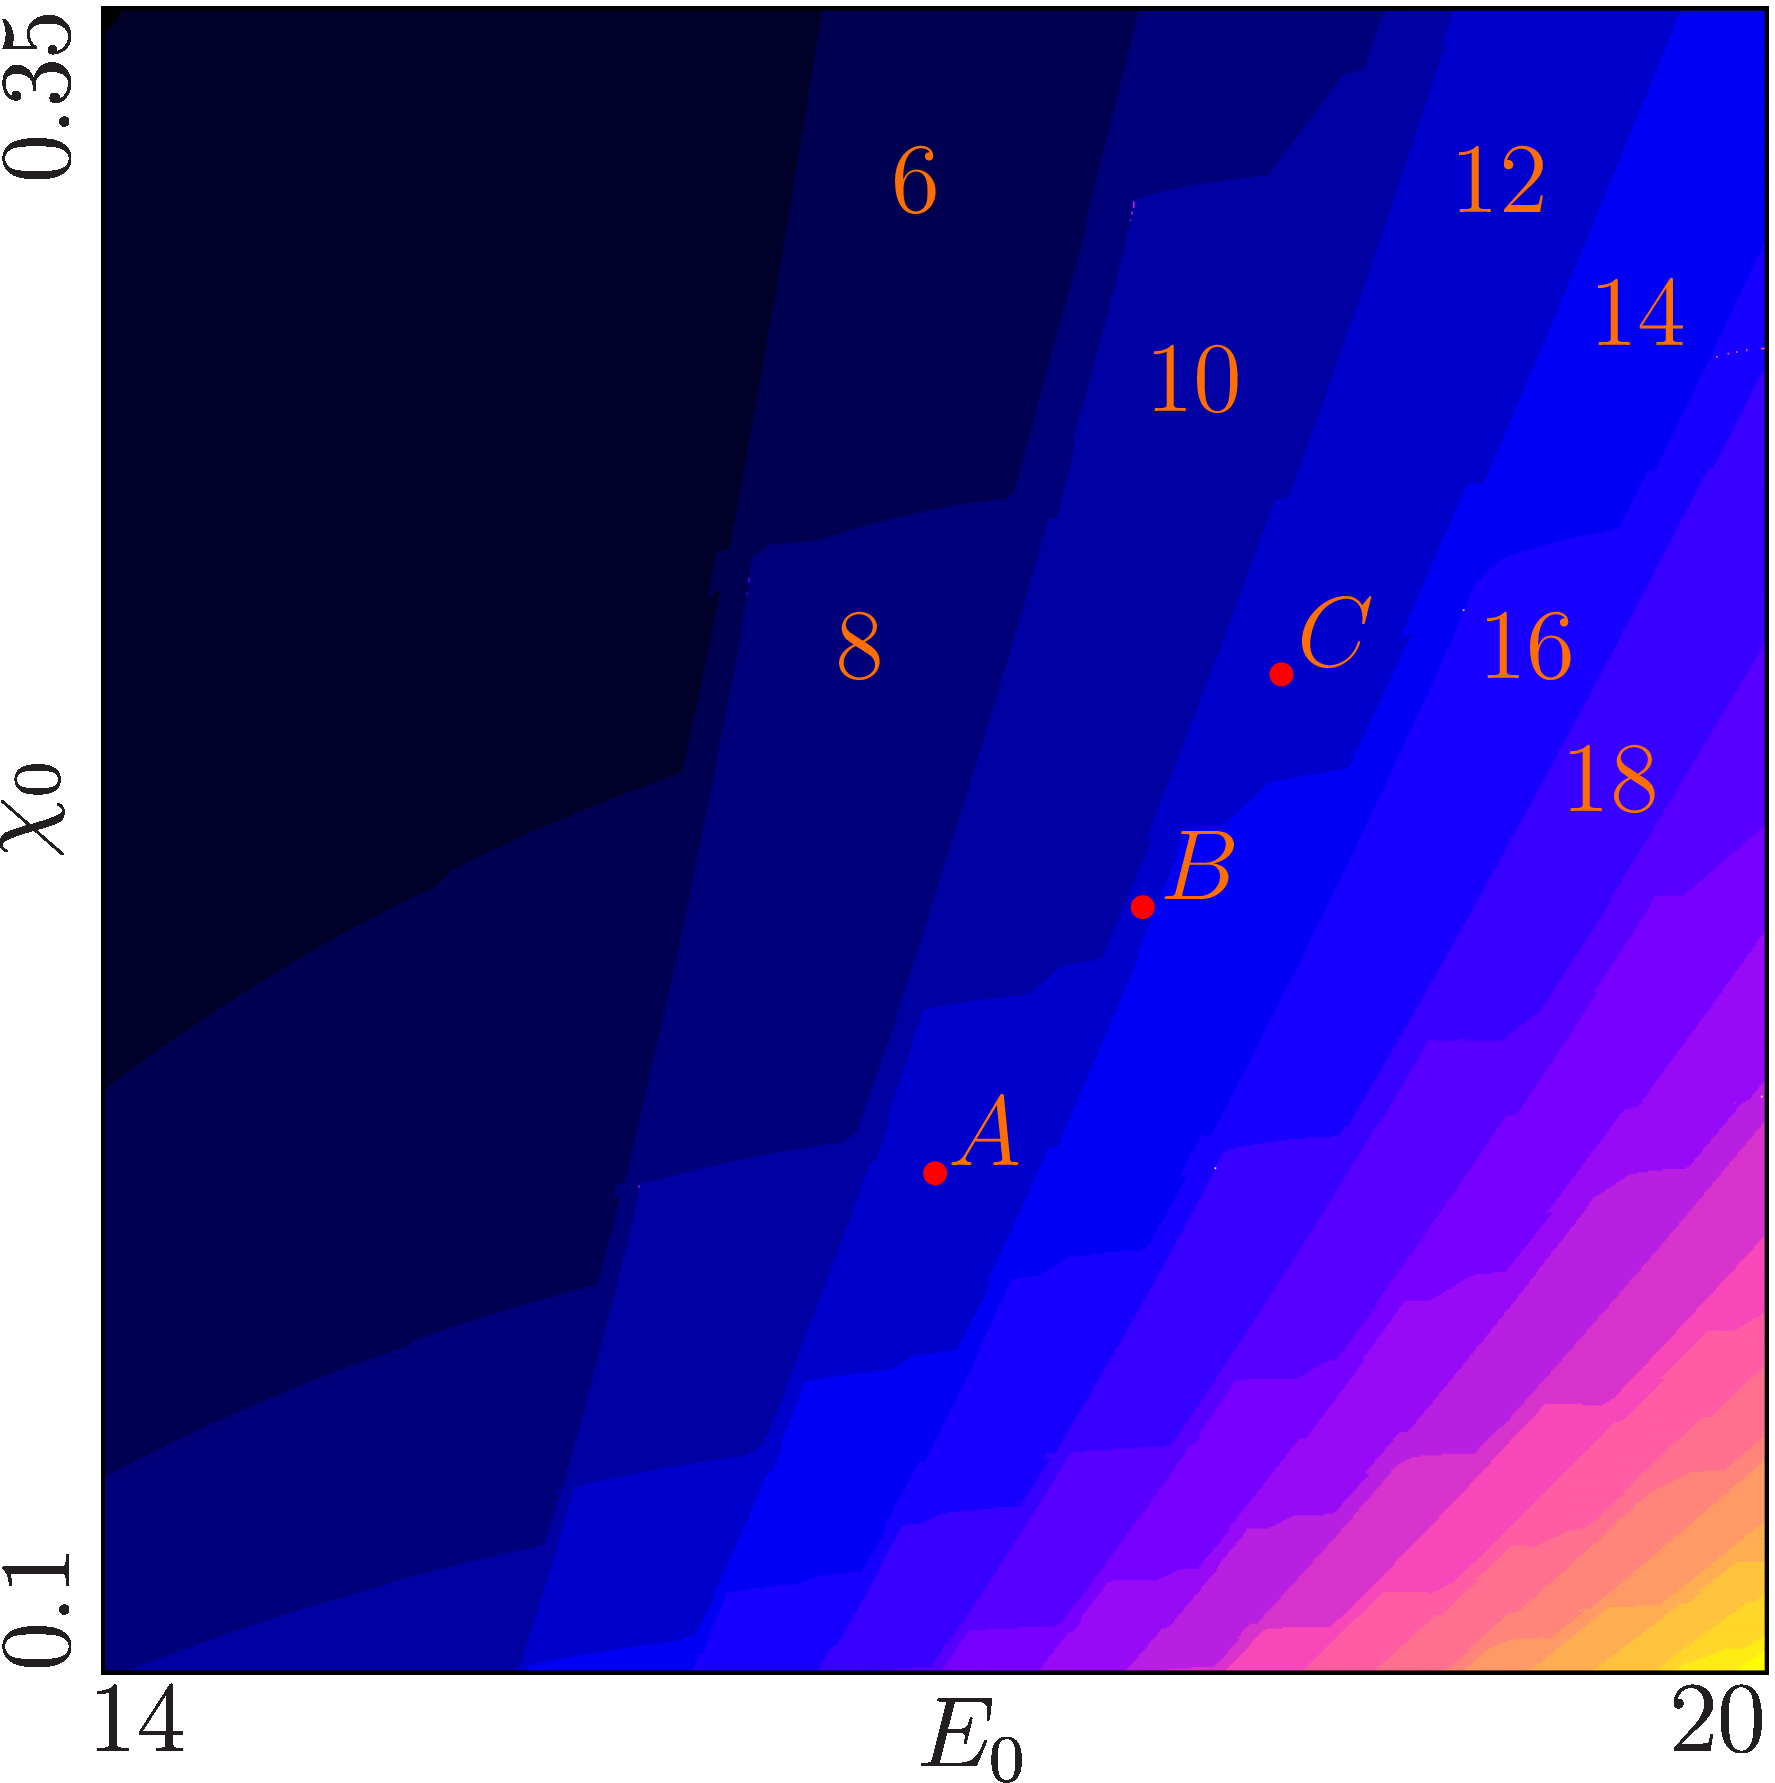
\includegraphics[width=0.4 \textwidth]{Figs/og_model_period.png}
			}{Original model}
			\qquad
			\stackunder[5pt]{
				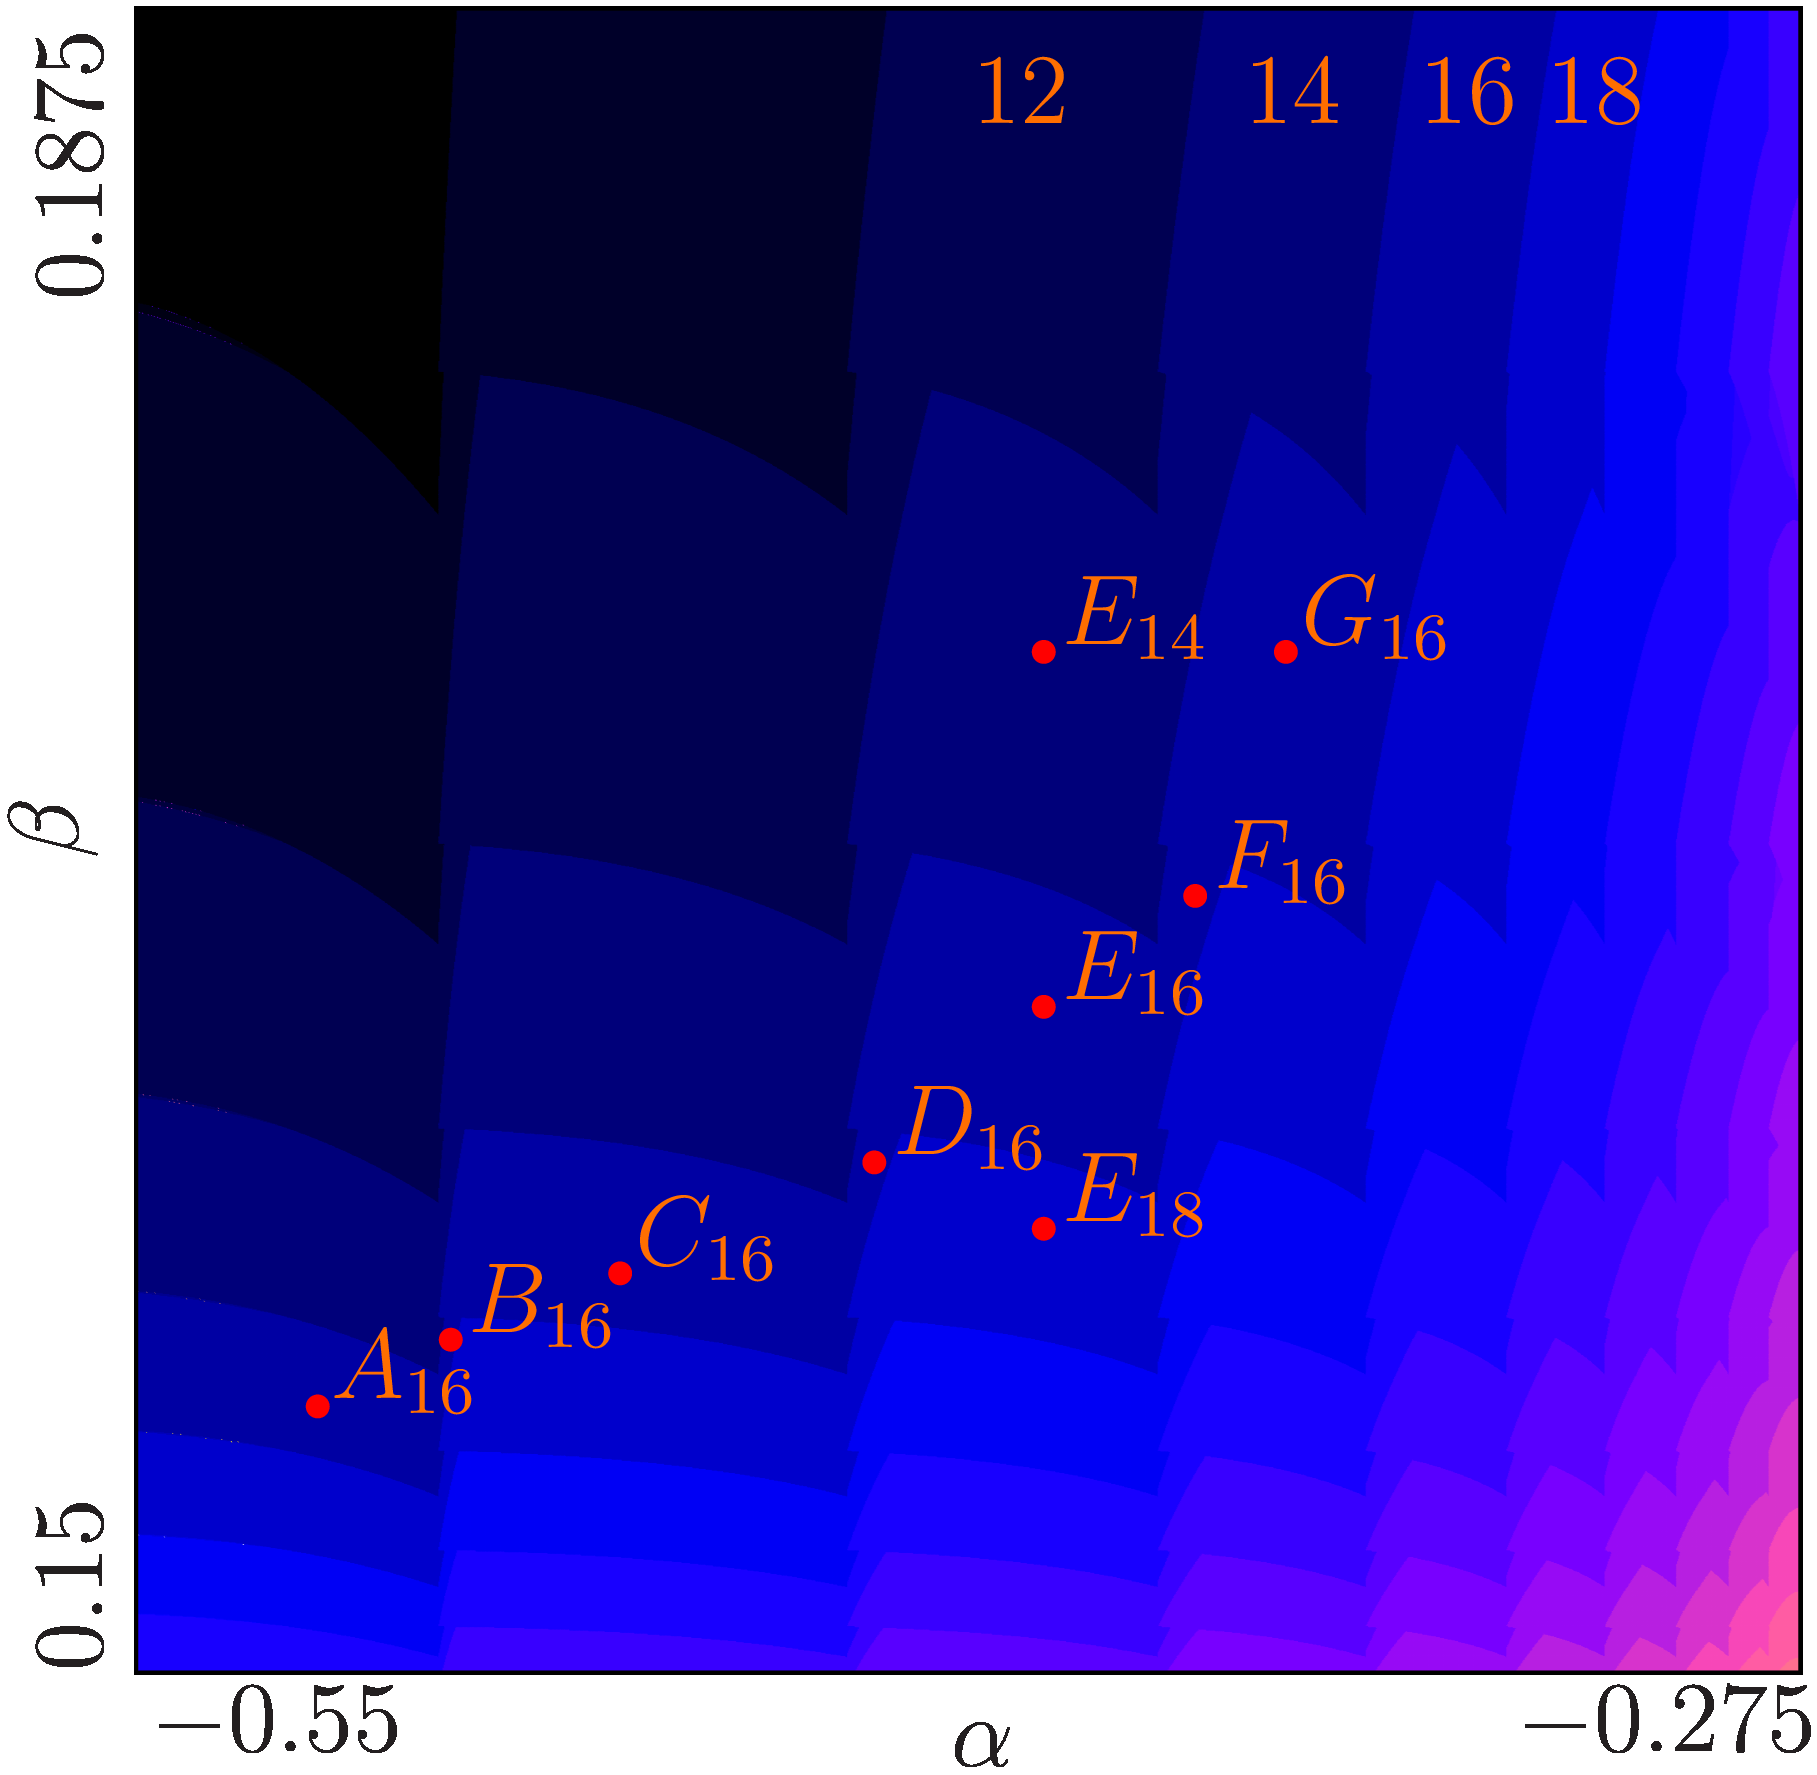
\includegraphics[width=0.41 \textwidth]{Figs/archetypal_model_period.png}
			}{Archetypal model}
		\end{figure}
	}
	\only<2>{
		\begin{figure}
			\centering
			\stackunder[5pt]{
				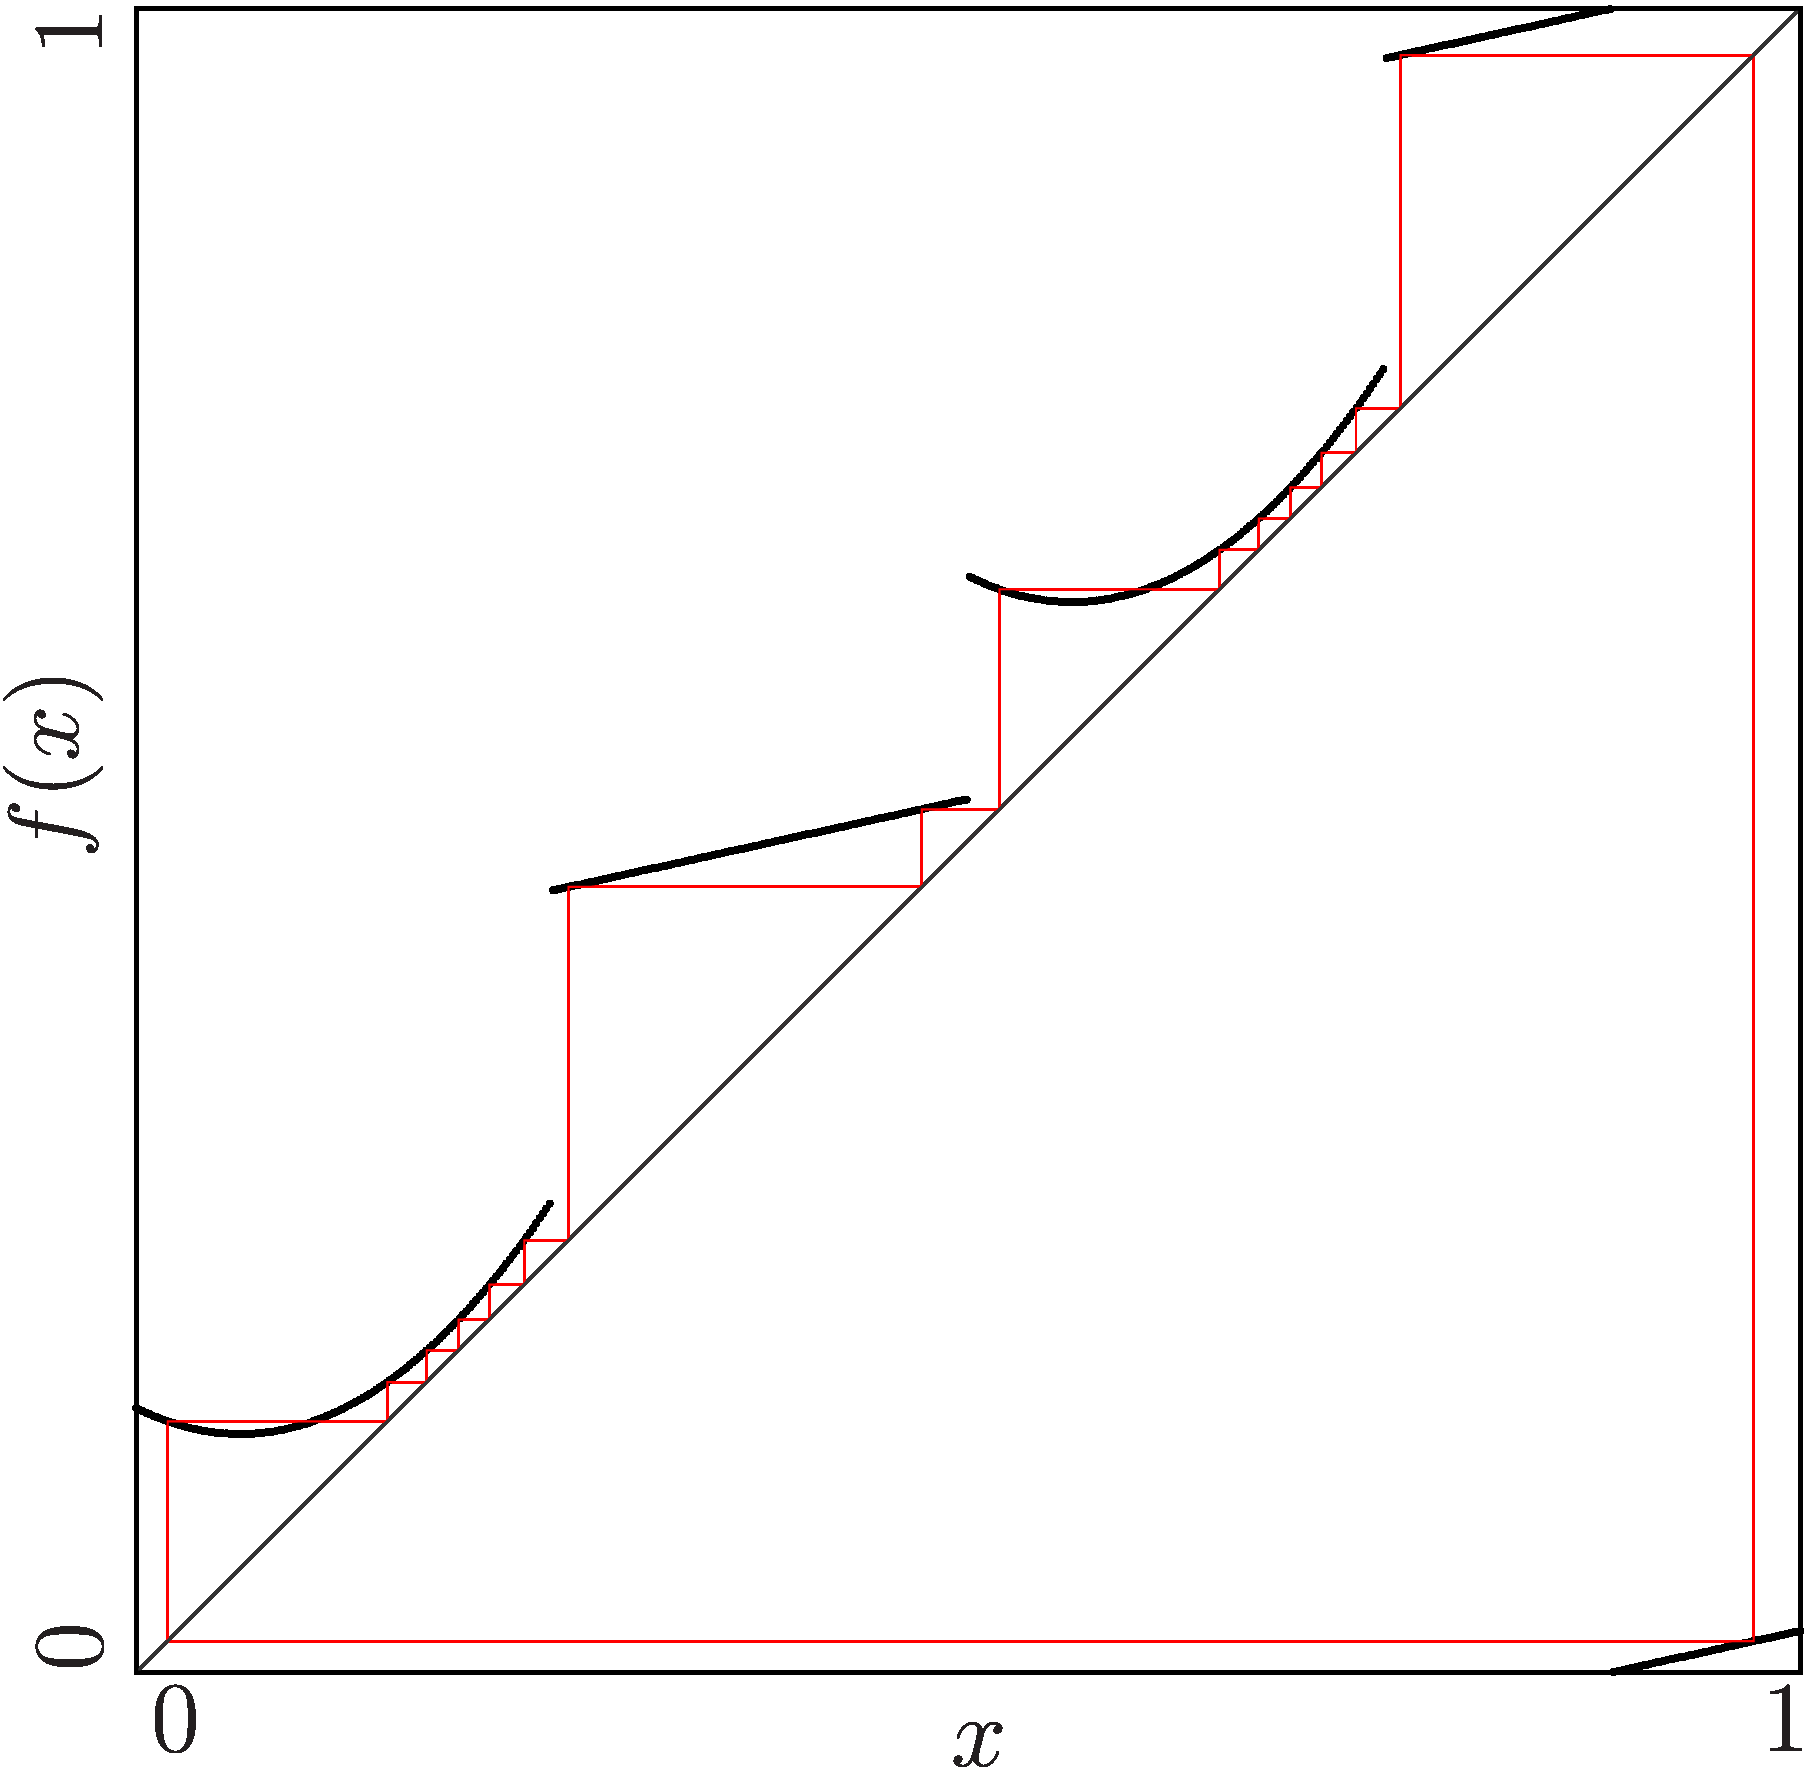
\includegraphics[width=0.3 \textwidth]{Figs/archetypal_model_cycle_c16.png}
			}{$C_{16}:\:\Cycle{\A^6\B^2\C^6\D^2}$}
			\stackunder[5pt]{
				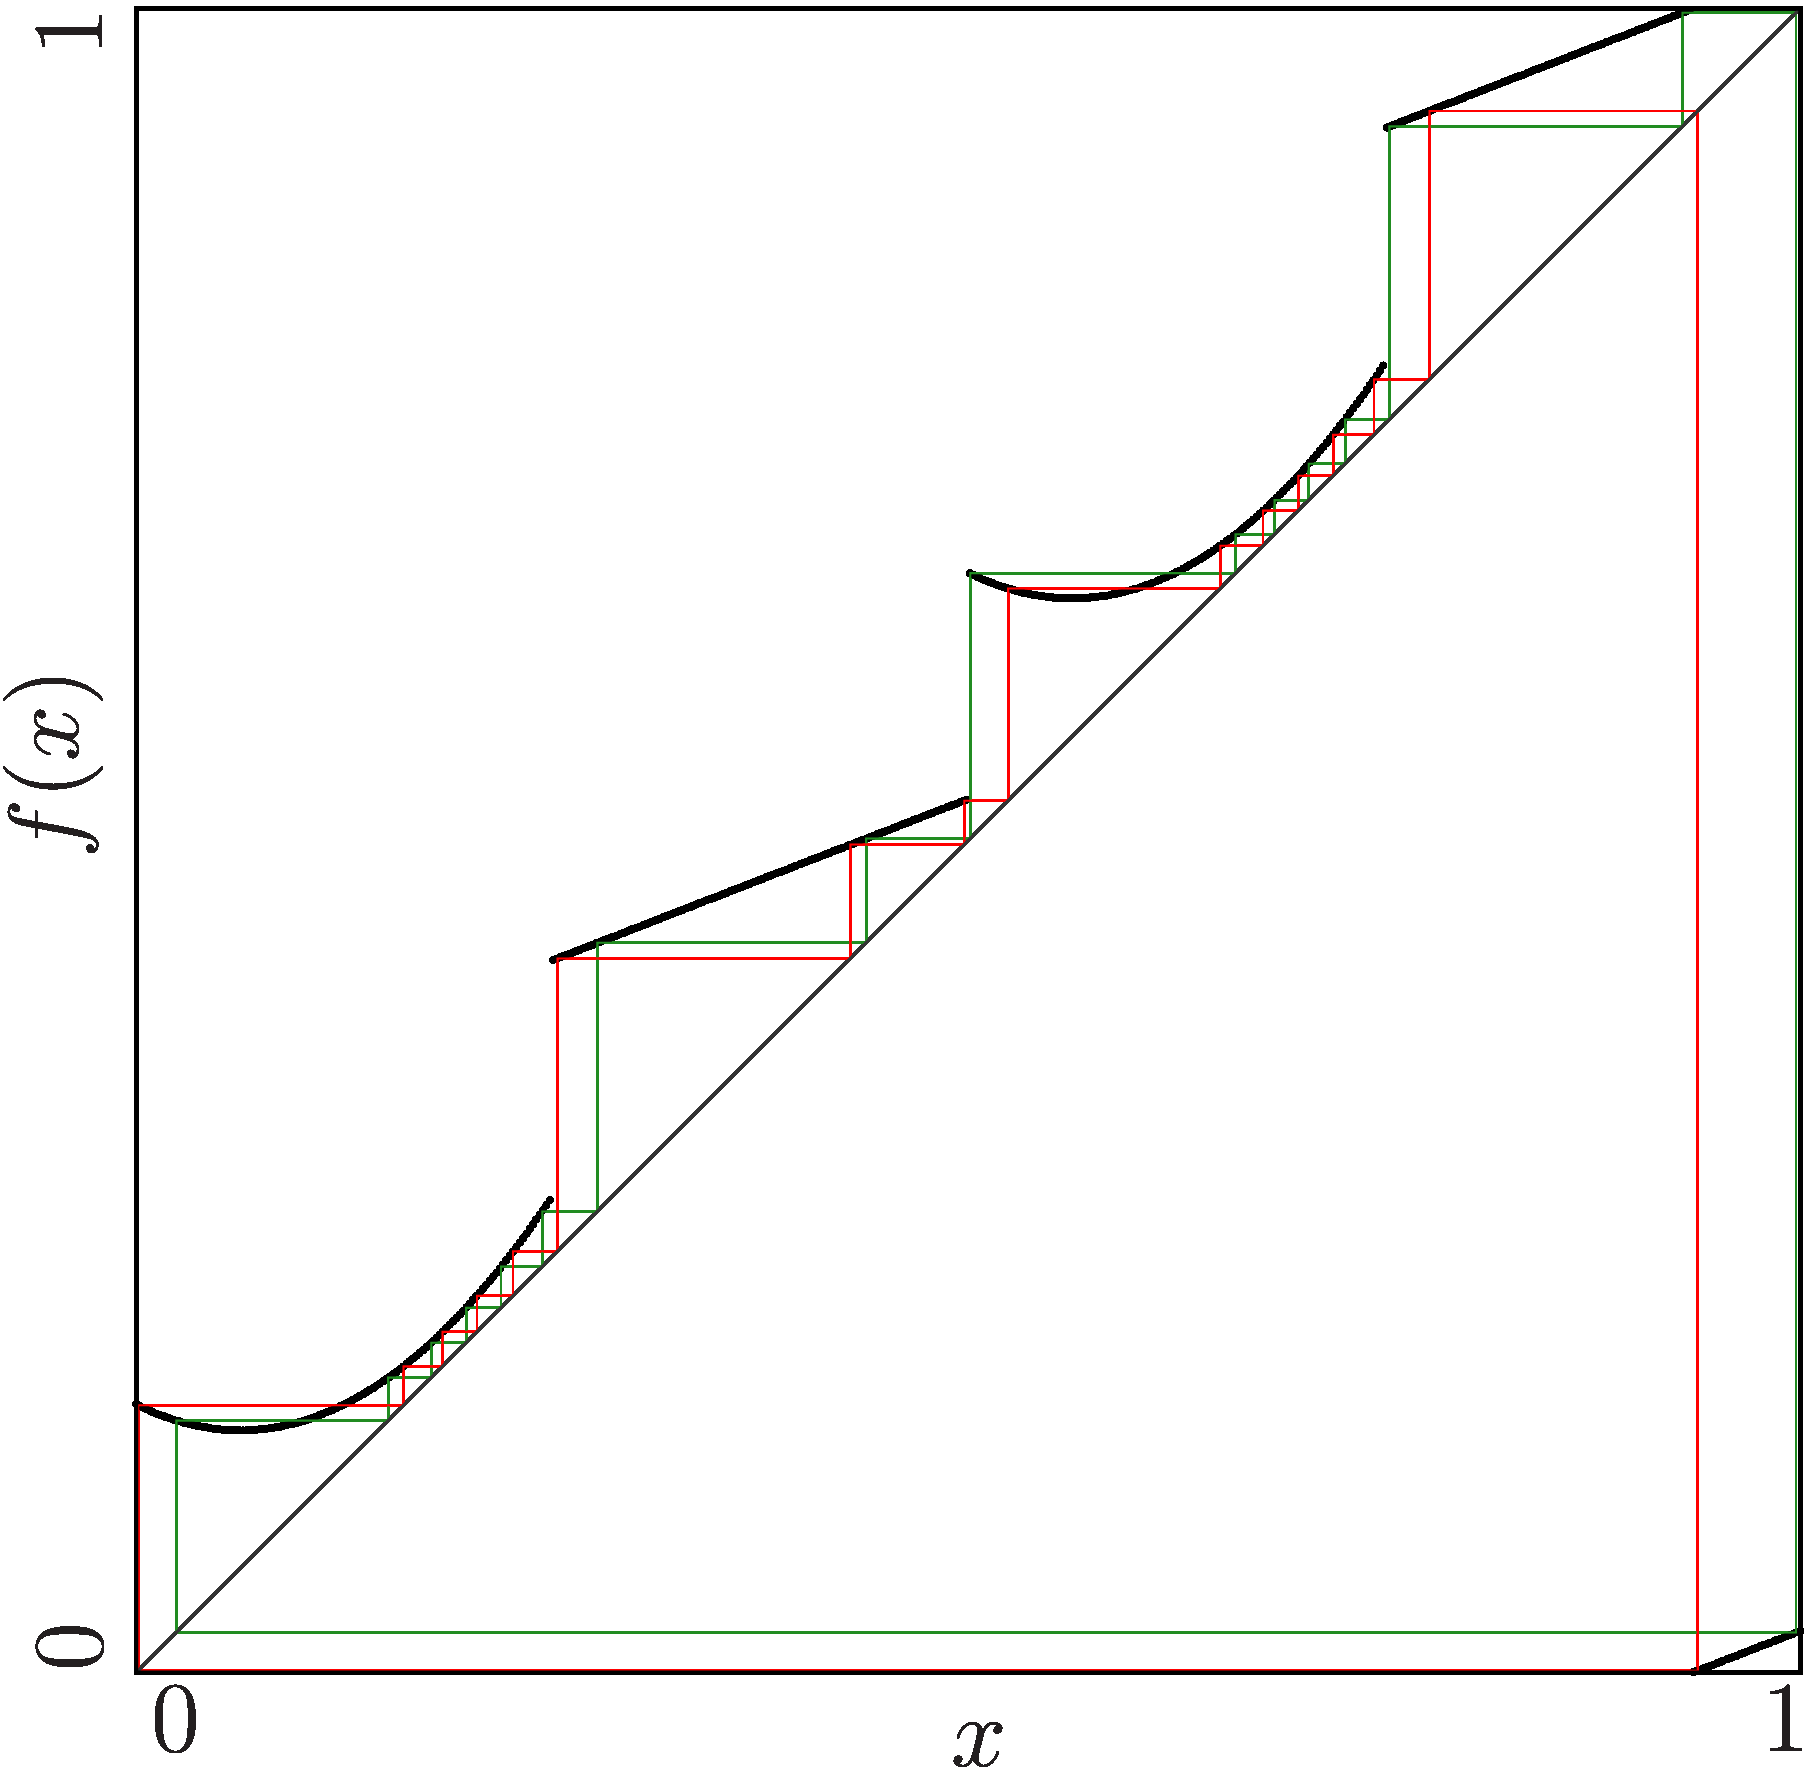
\includegraphics[width=0.3 \textwidth]{Figs/archetypal_model_cycle_d16.png}
			}{$D_{16}:\:\Cycle{\A^6\B^2\C^5\D^3},\Cycle{\A^5\B^3\C^6\D^2}$}
			\stackunder[5pt]{
				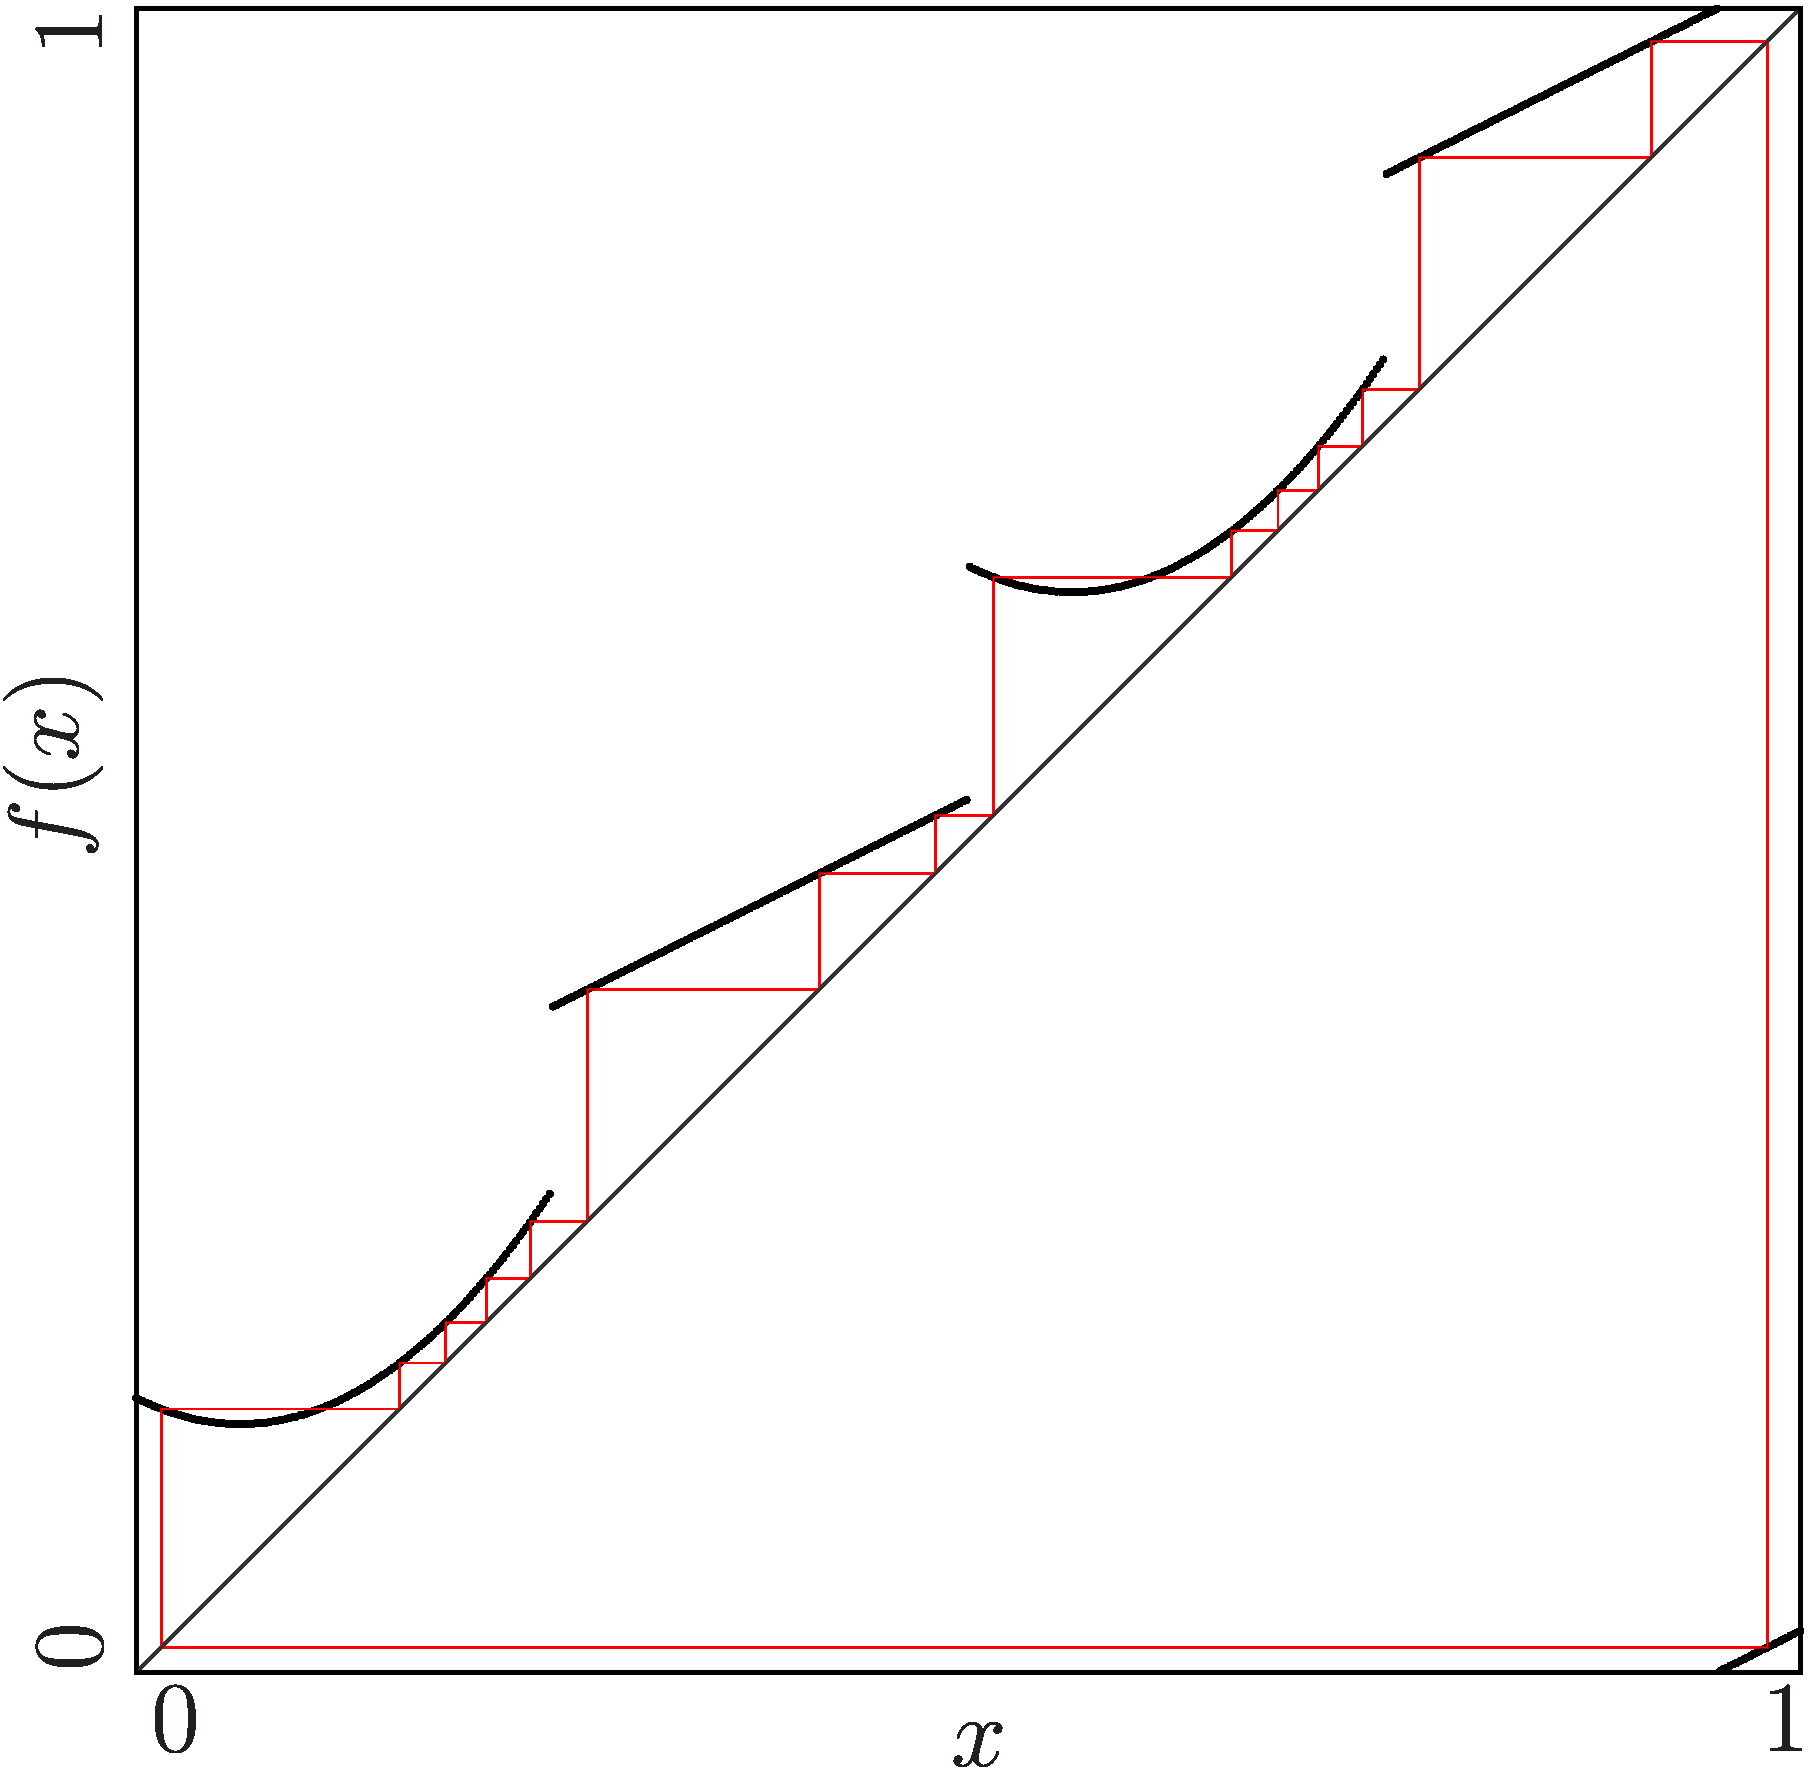
\includegraphics[width=0.3 \textwidth]{Figs/archetypal_model_cycle_e16.png}
			}{$E_{16}:\:\Cycle{\A^5\B^3\C^5\D^3}$}
		\end{figure}
	}
\end{frame}

\begin{frame}{Archetypal Model Equations}
	\vspace{-1.0em}
	\only<1>{
		\begin{align*}
			x_{n+1} = f(x_n) \mod 1
		\end{align*}
		\begin{align*}
			f(x) & = \begin{cases}
				         g(x)                                        & \text{ if } x < \frac{1}{2} \\
				         g\left(x - \frac{1}{2}\right) + \frac{1}{2} & \text{ else}
			         \end{cases}
		\end{align*}
		\begin{align*}
			g(x) & = \begin{cases}
				         g_L(x) = a_L \cdot x^2 + b_L \cdot x + c_L & \text{ if } x < \frac{1}{4} \\
				         g_R(x) = b_R \cdot x + c_R                 & \text{ else}
			         \end{cases}
		\end{align*}
	}
	\only<2>{
		\begin{columns}
			\begin{column}{.7 \textwidth}
				Fixed parameters:
				\begin{align*}
					a_L = 4 \text{ and } b_L = -\tfrac{1}{2}
				\end{align*}
				Variable parameters
				\begin{align*}
					 & c_L, b_R, c_R                                                                                                              \\
					\text{where} \qquad
					 & c_L = \beta,                                                                                                               \\
					 & b_R = -4 \cdot g_R\left(\tfrac{1}{4}\right) + 4 \cdot g_R\left(\tfrac{1}{2}\right),                                        \\
					 & c_R = 2 \cdot g_R\left(\tfrac{1}{4}\right) - 1 \cdot g_R\left(\tfrac{1}{2}\right),                                         \\[1em]
					\text{and} \qquad
					 & g_R\left(\tfrac{1}{4}\right) = \alpha, \text{and } g_R\left(\tfrac{1}{2}\right) = \tfrac{1}{2} + \epsilon \text{ is fixed}
				\end{align*}
			\end{column}
			\begin{column}{.3 \textwidth}
				\begin{figure}
					\centering
					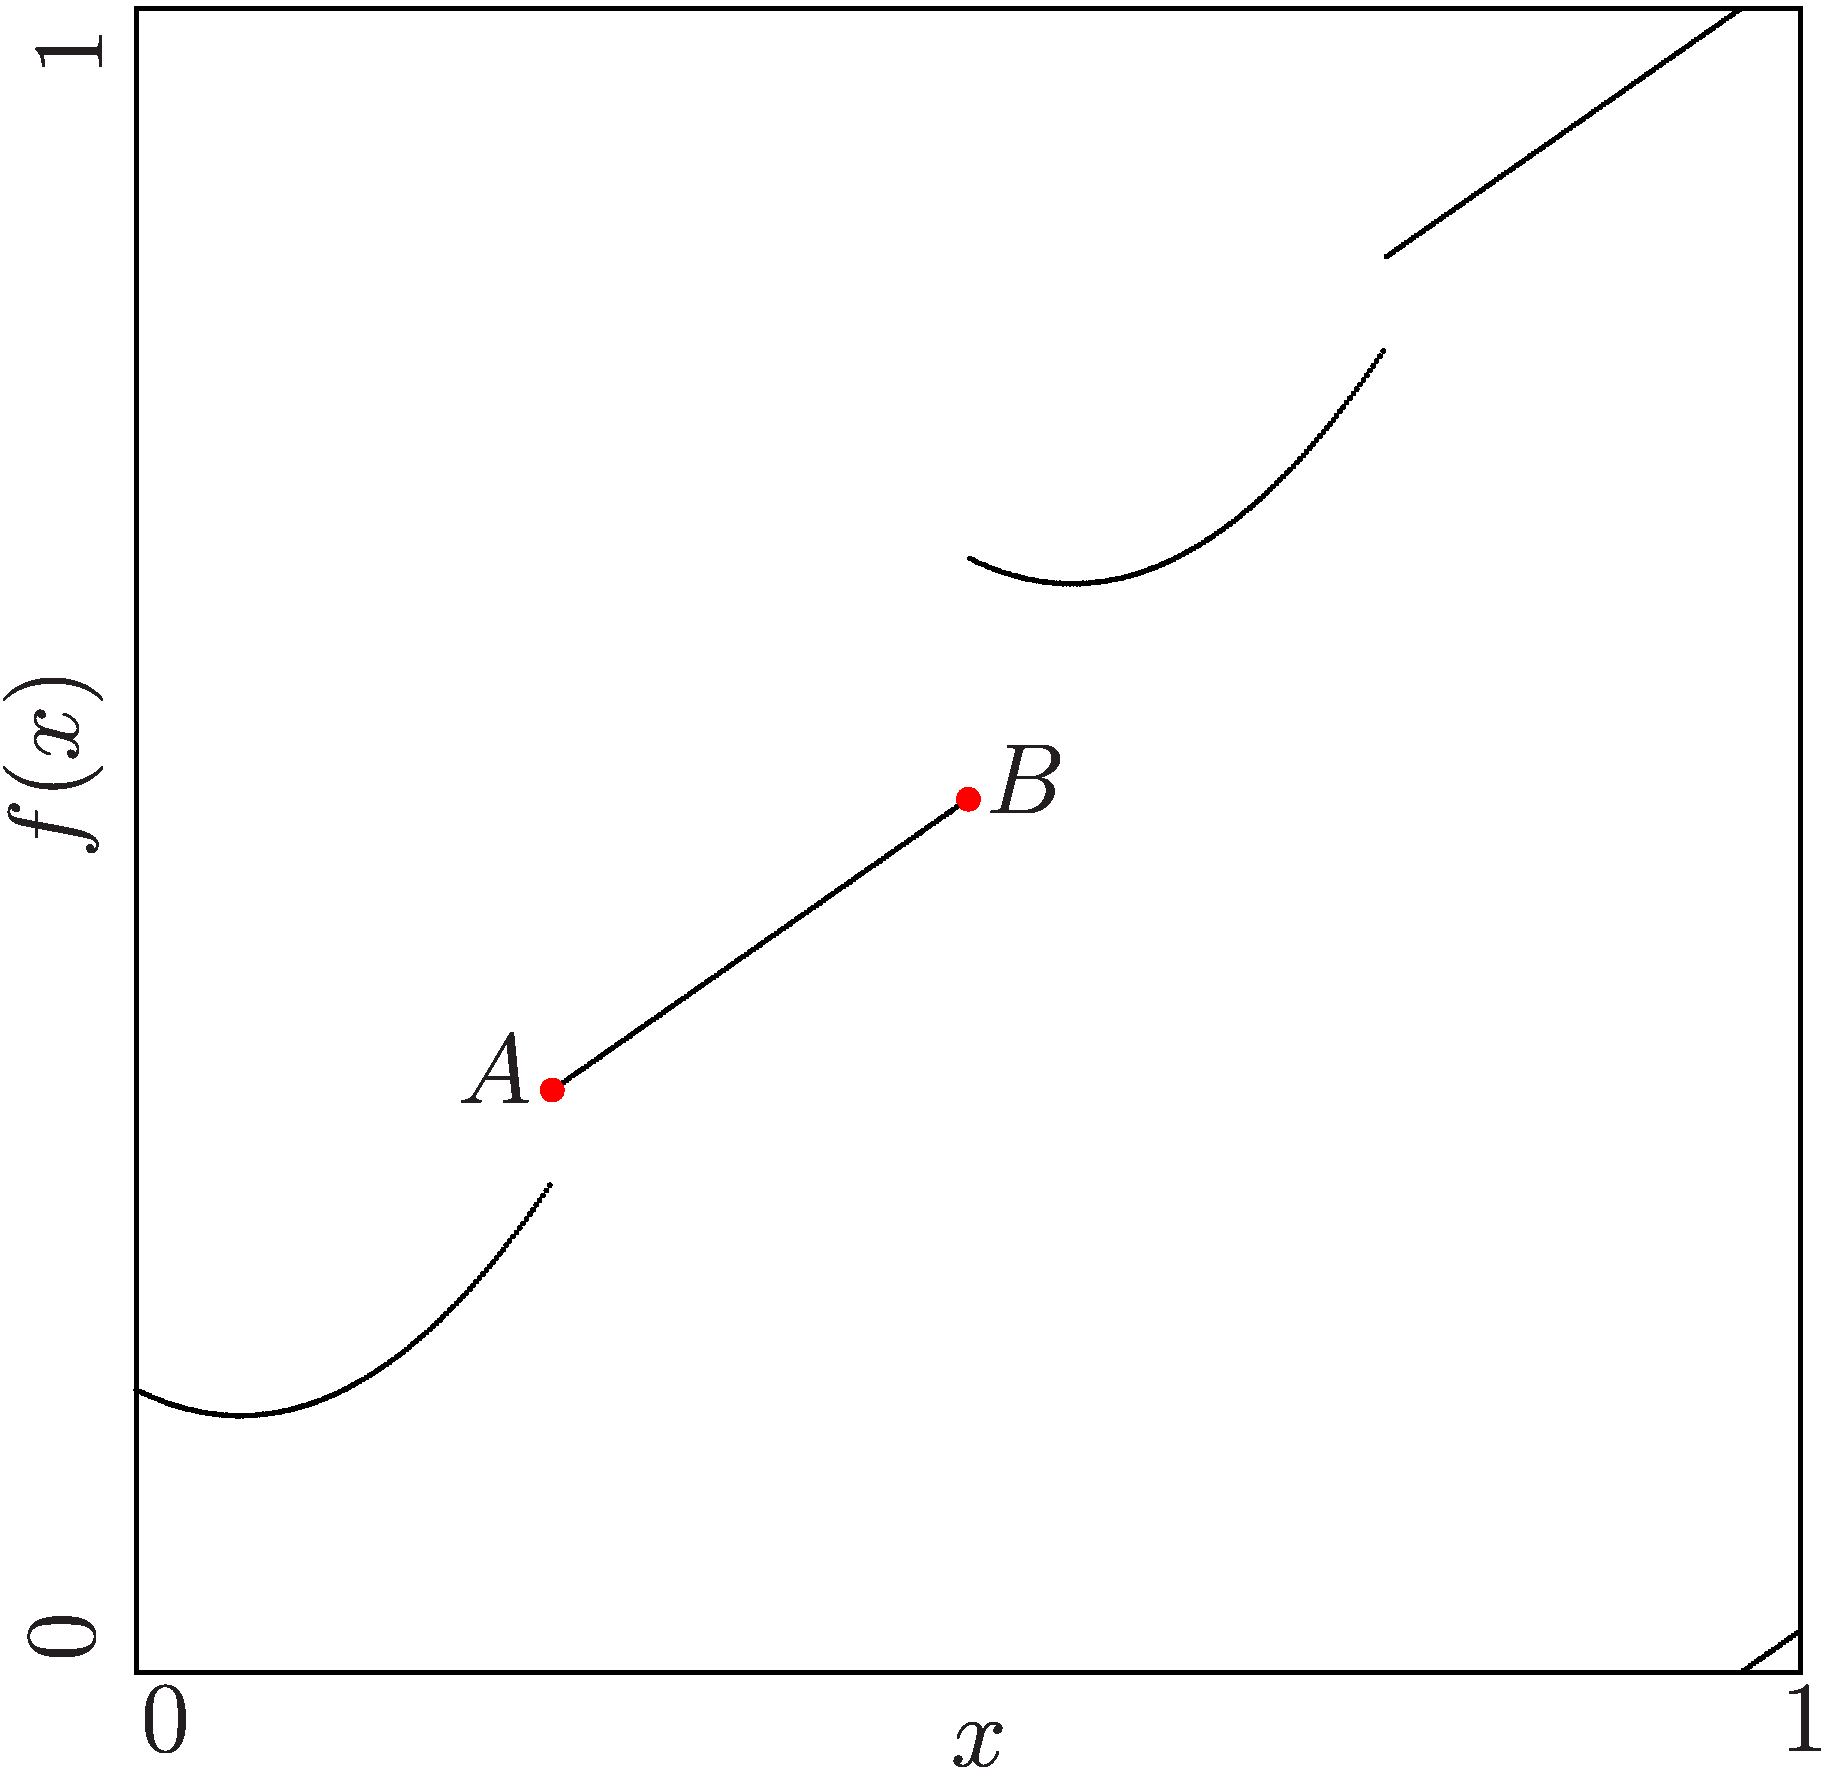
\includegraphics[height=.5 \textheight]{Figs/archetypal_model_parameter_effects_illustration.png}
				\end{figure}
			\end{column}
		\end{columns}
	}
\end{frame}

\begin{frame}{Archetypal Model Results}
	\begin{itemize}
		\item Description of the bifucation structure
		\item Explanation of coexisting cycles via the symmetry
		\item Explanation of double border collisions via the symmetry
		\item Discovery of 4 coexisting cycles not discovered in the original model
		      \begin{itemize}
			      \item Confirmation of 4 coexisting cycles in the original model
		      \end{itemize}
	\end{itemize}
\end{frame}

\begin{frame}{Period-Adding?}
	\vspace{-1em}
	\begin{itemize}
		\item Chains overlap
		\item What happens, when they no longer overlap?
		      \vspace{1em}
		\item Prediction: Period-Adding
		      %\item Turns up often
		      %\item E.g. Edge of main bubble of mandelbrot set
	\end{itemize}
	\begin{figure}
		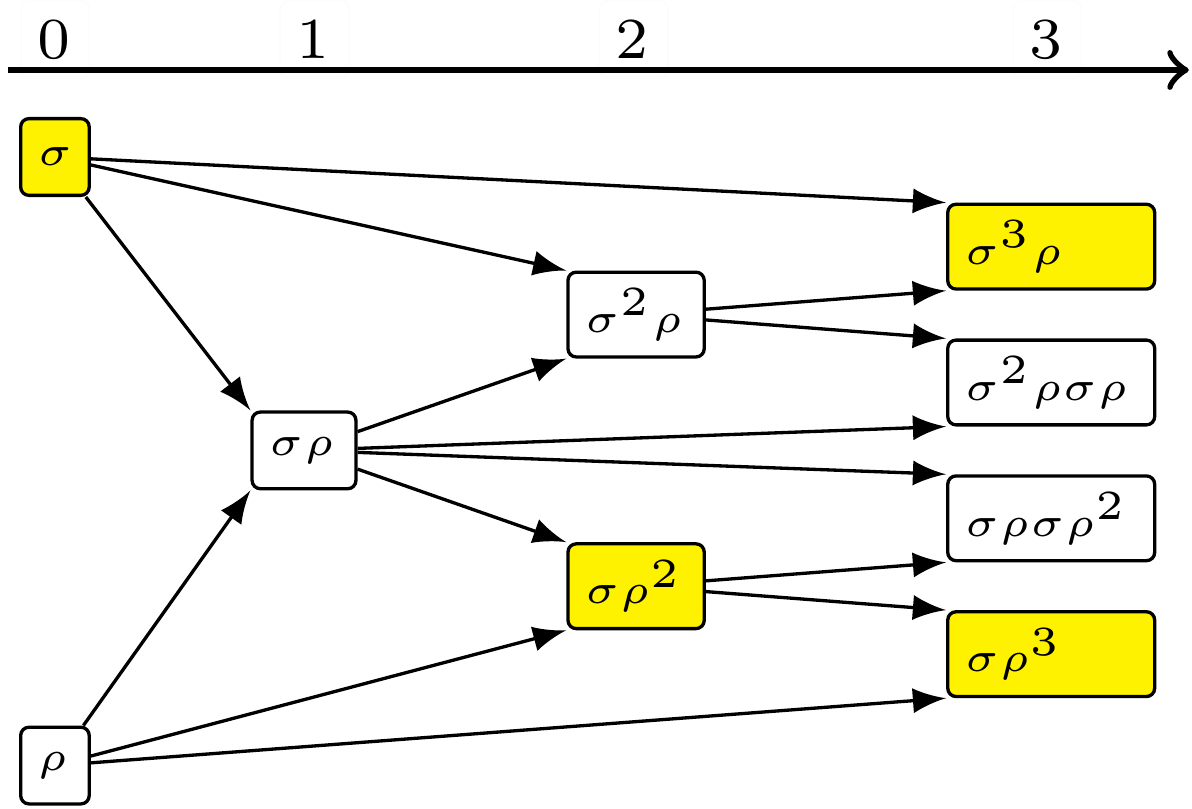
\includegraphics[height=.5 \textheight]{Figs/Trees/ClassicalAdding/adding.png}
	\end{figure}
\end{frame}

\begin{frame}{Archetypal Model with Different Parameters}
	\only<1>{
		\begin{figure}
			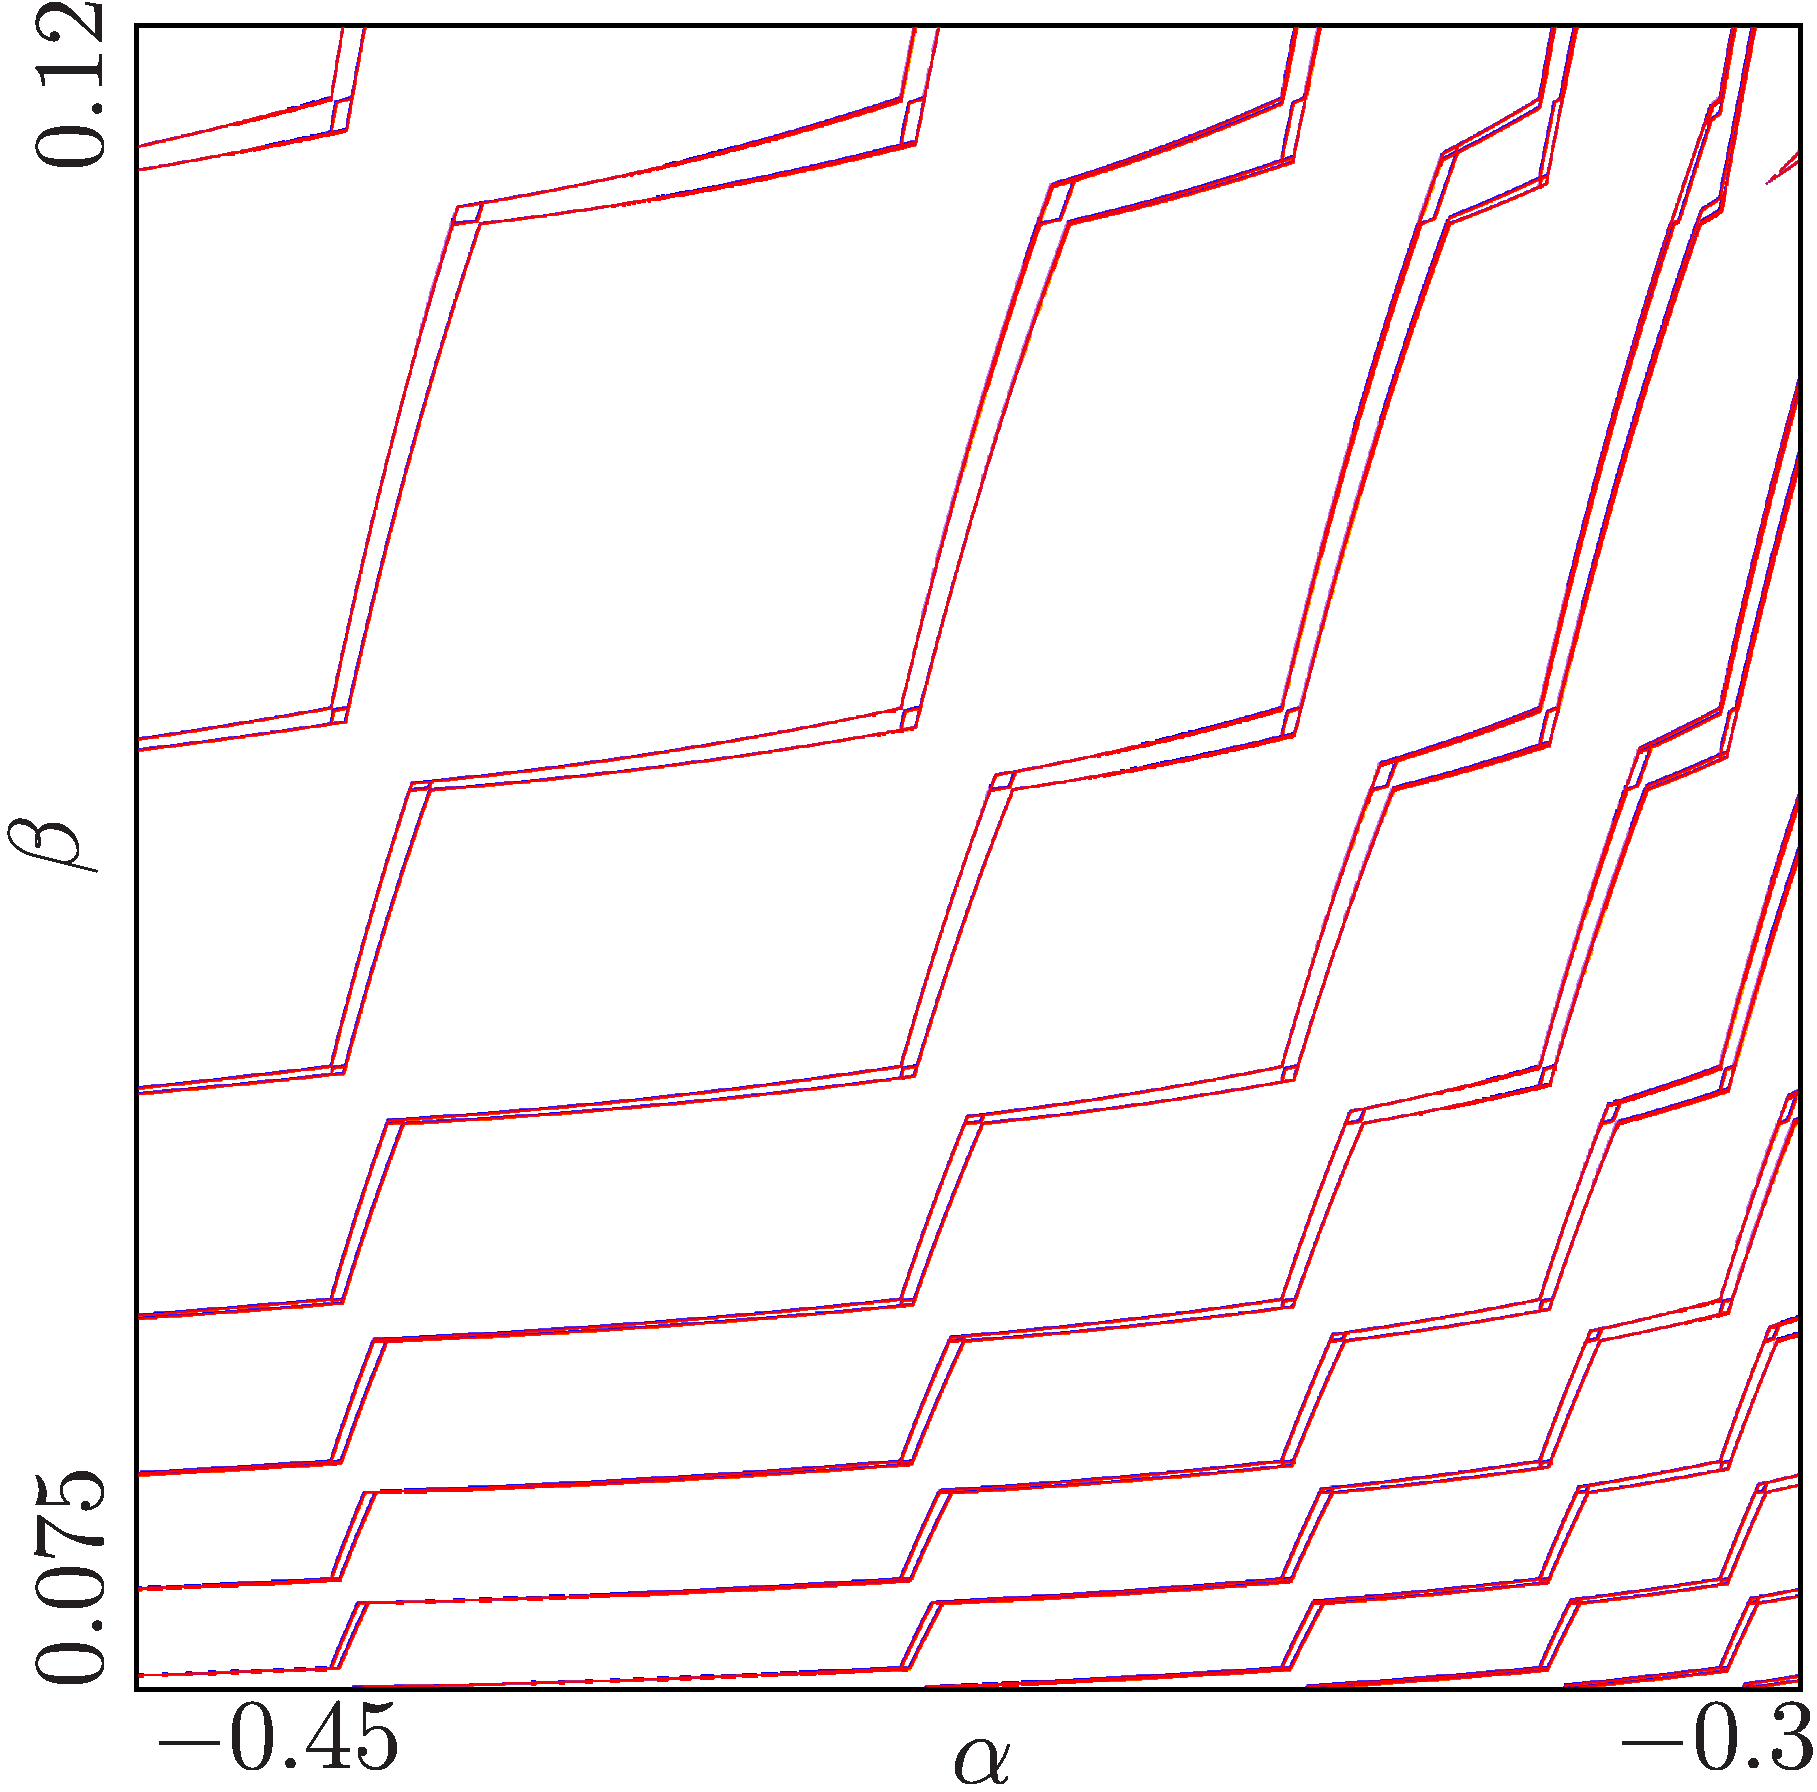
\includegraphics[width=.4 \textwidth]{Figs/archetypal_model_regions_drifting_apart.png}
			\quad
			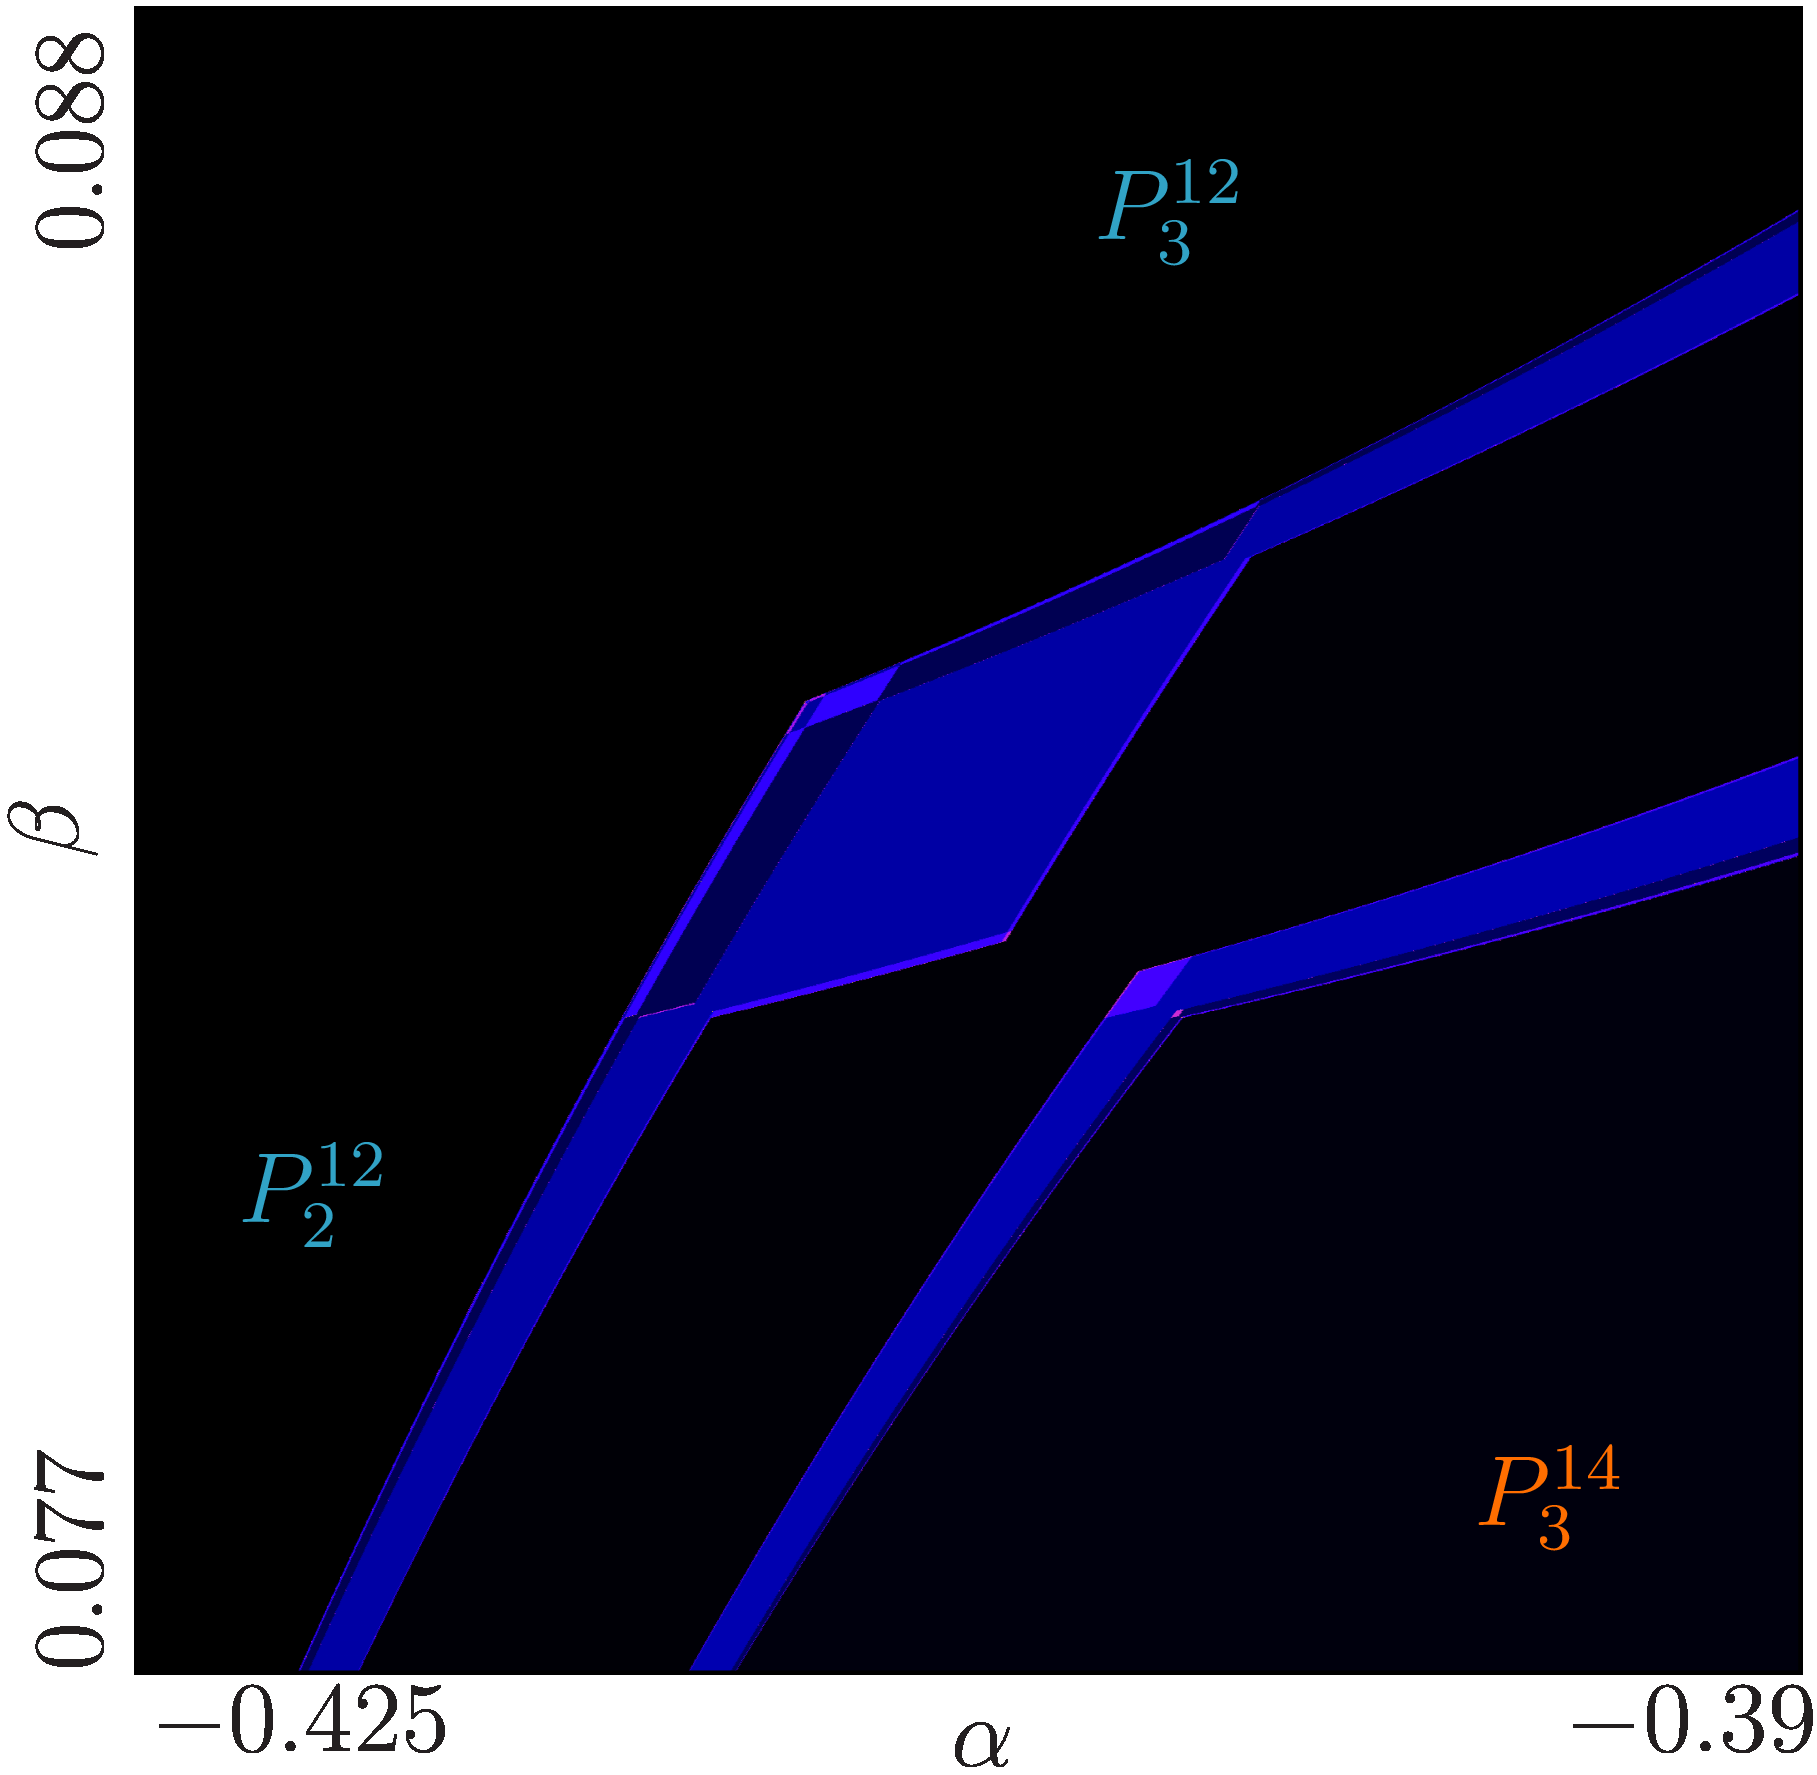
\includegraphics[width=.4 \textwidth]{Figs/archetypal_model_adding_like_period_corner.png}
		\end{figure}
	}
	\only<2>{
		\vspace{-1em}
		\begin{figure}
			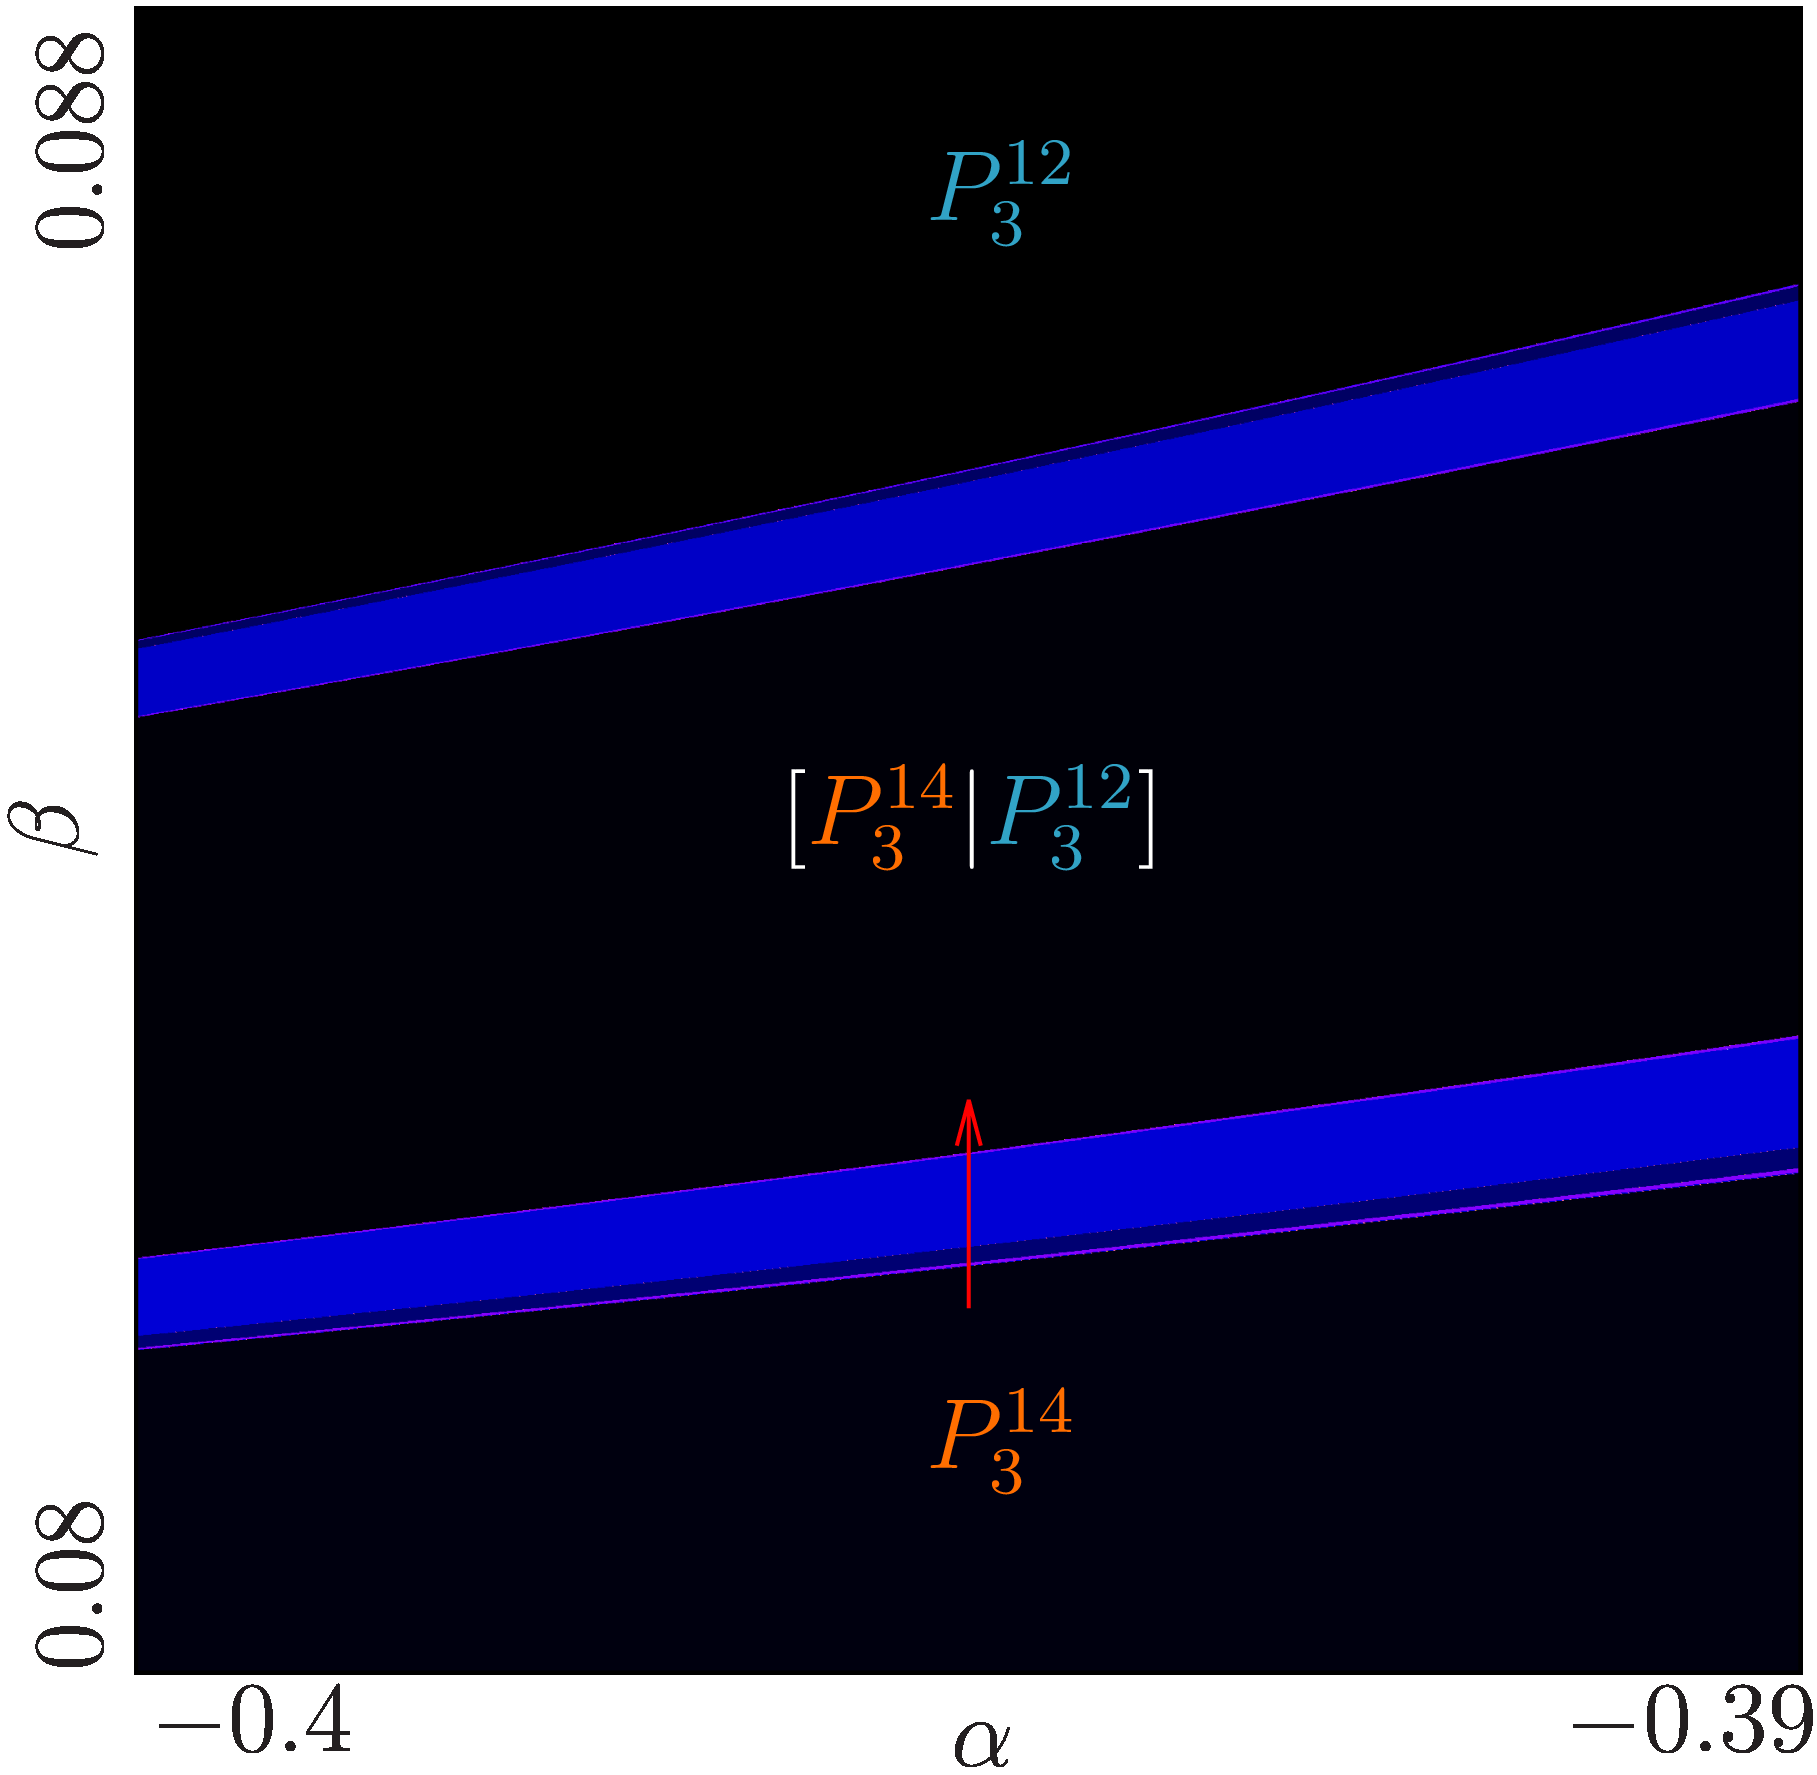
\includegraphics[width=.4 \textwidth]{Figs/archetypal_model_full_add_hor_2D.png}
			\qquad
			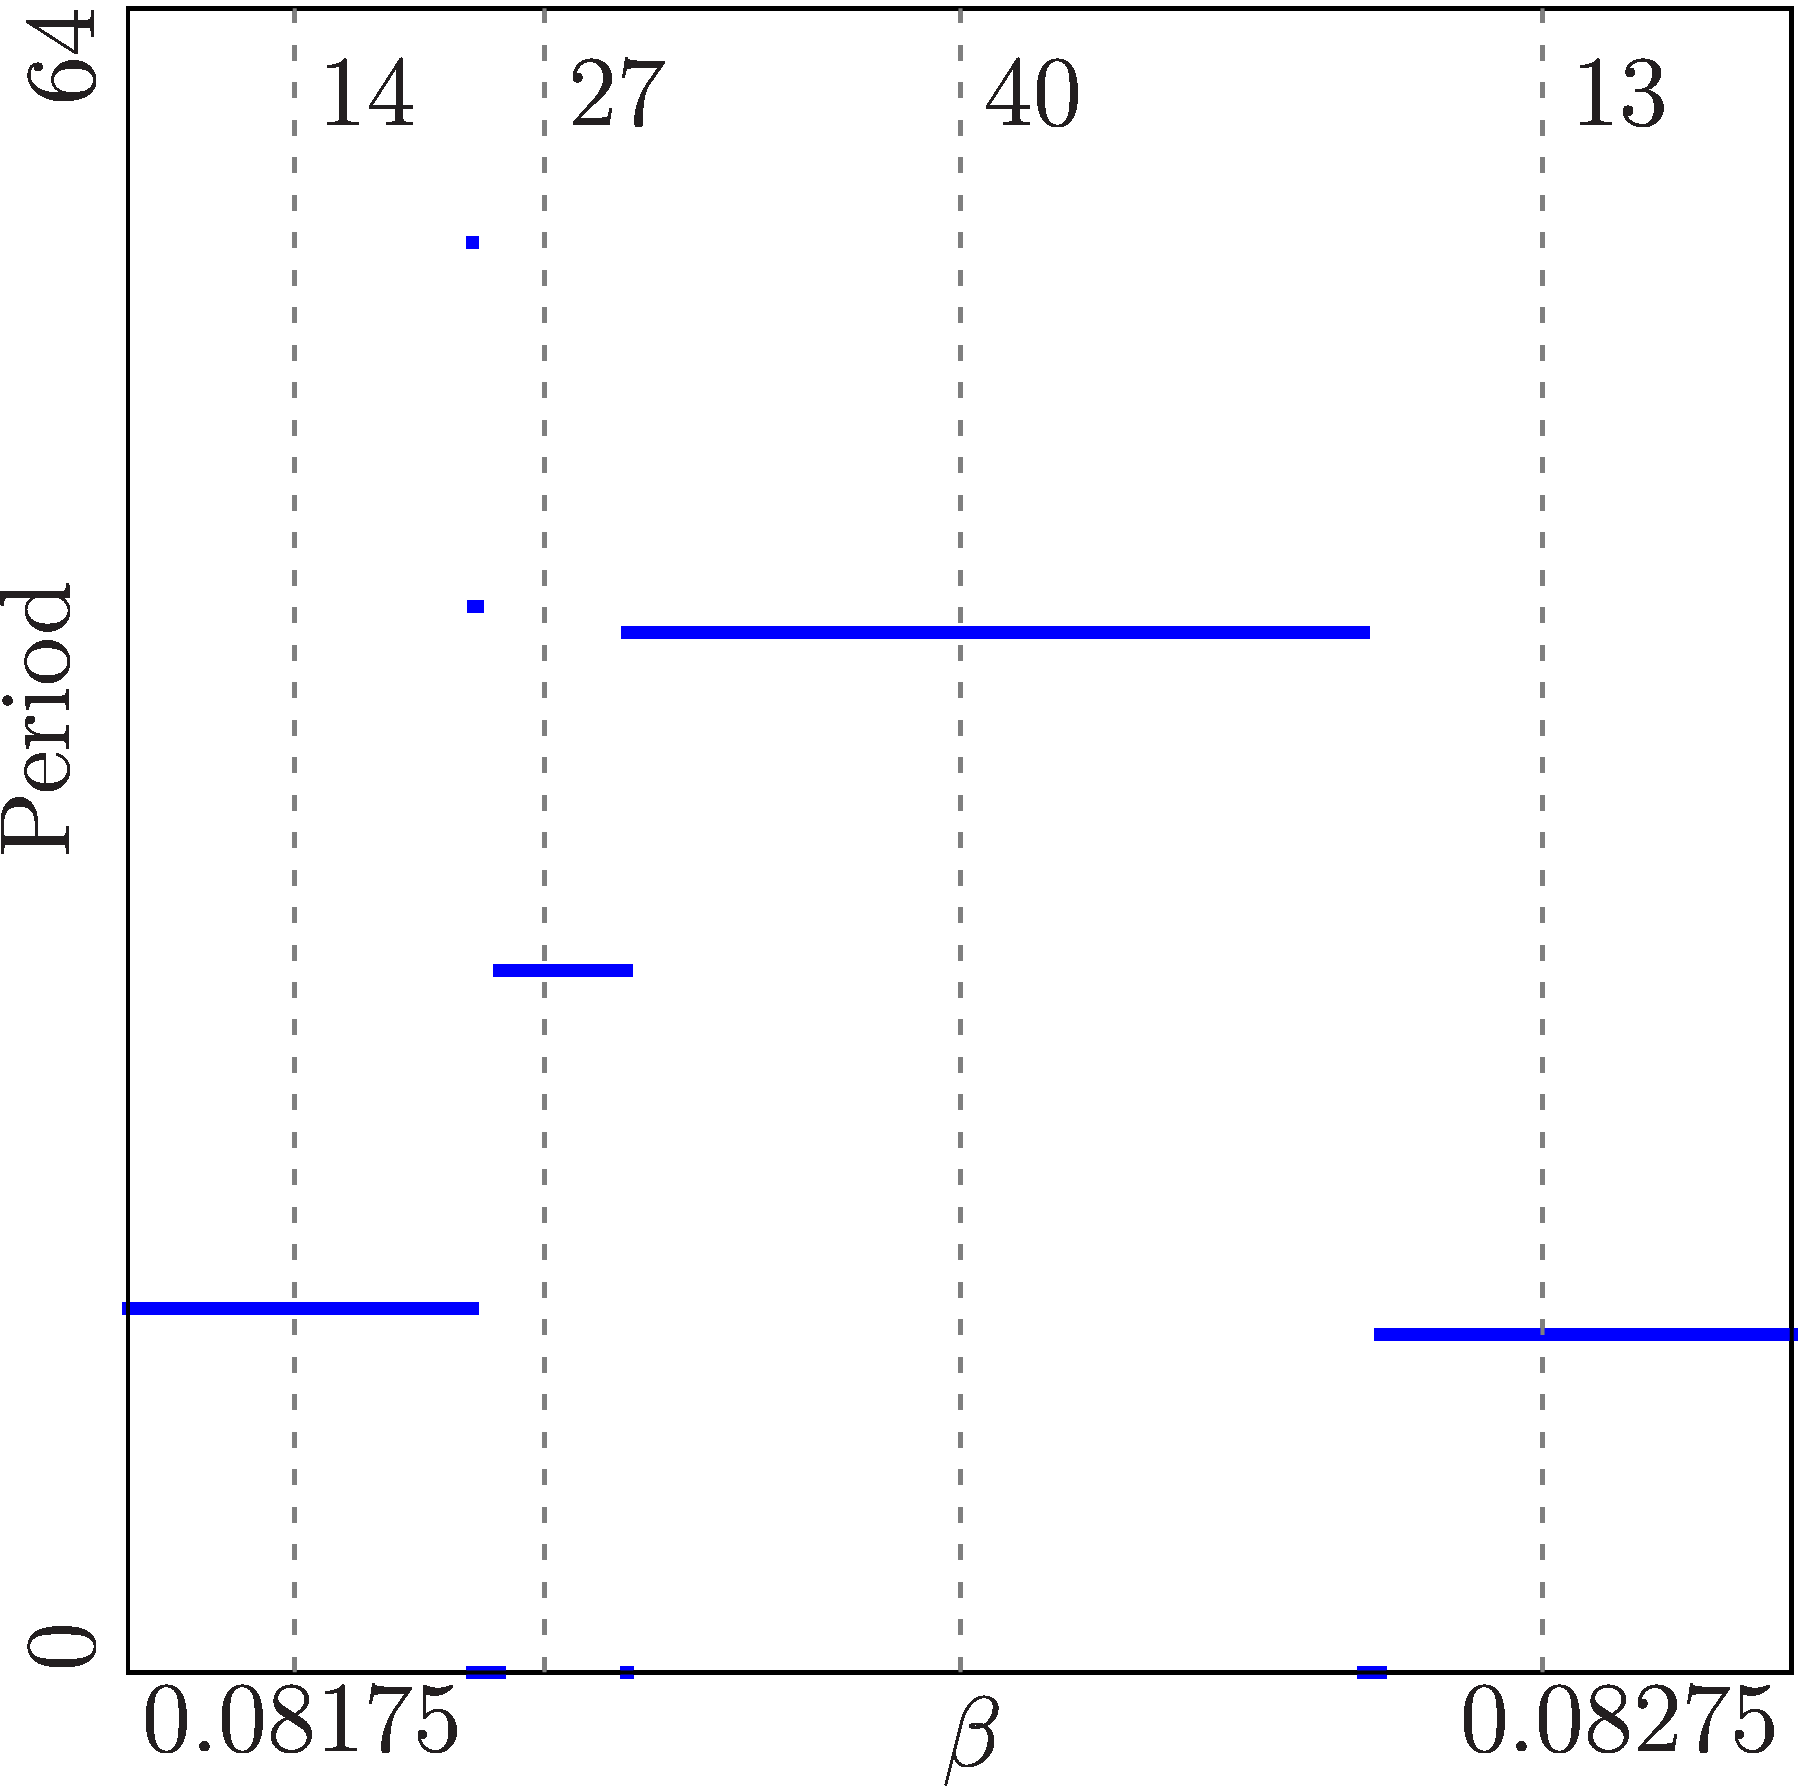
\includegraphics[width=.4 \textwidth]{Figs/archetypal_model_full_add_hor_1D.png}
		\end{figure}
	}
	\only<3>{
		\vspace{-1em}
		\begin{figure}
			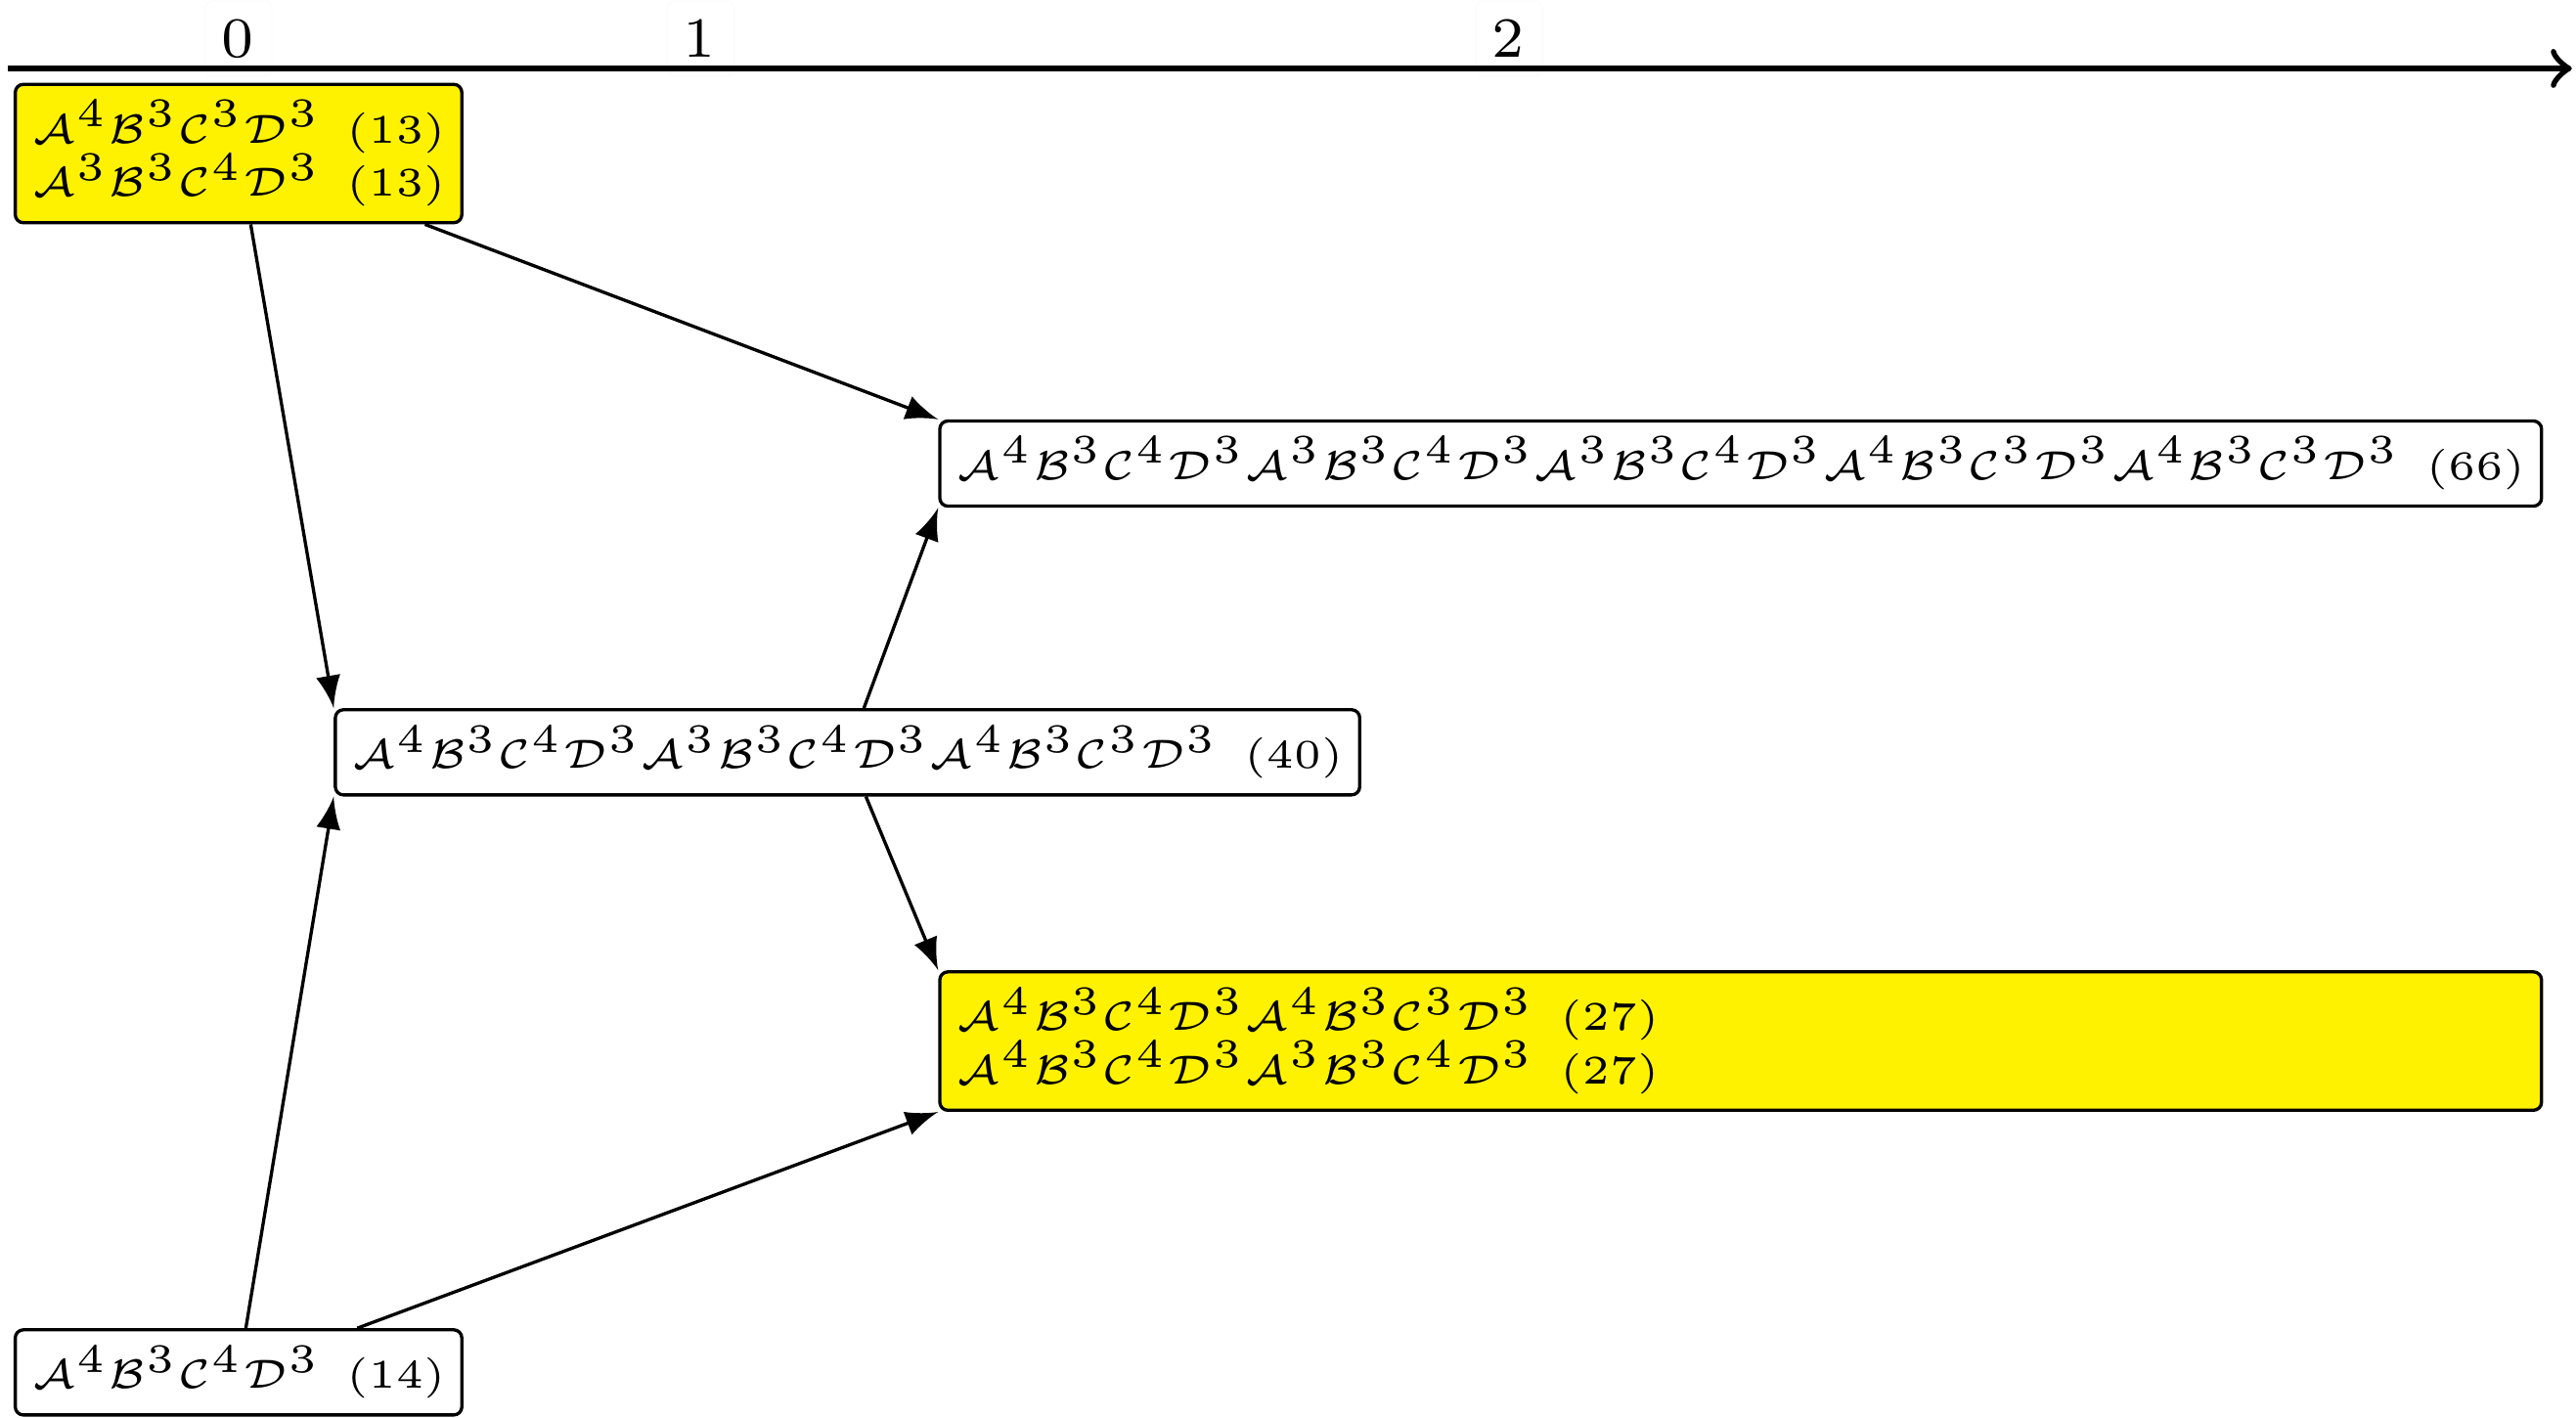
\includegraphics[width=.7 \textwidth]{Figs/Trees/FullArchetypal/adding.png}
		\end{figure}
	}
\end{frame}

\begin{frame}{Halved Model}
	\vspace{-1em}
	\begin{columns}
		\begin{column}{.4 \textwidth}
			\begin{figure}
				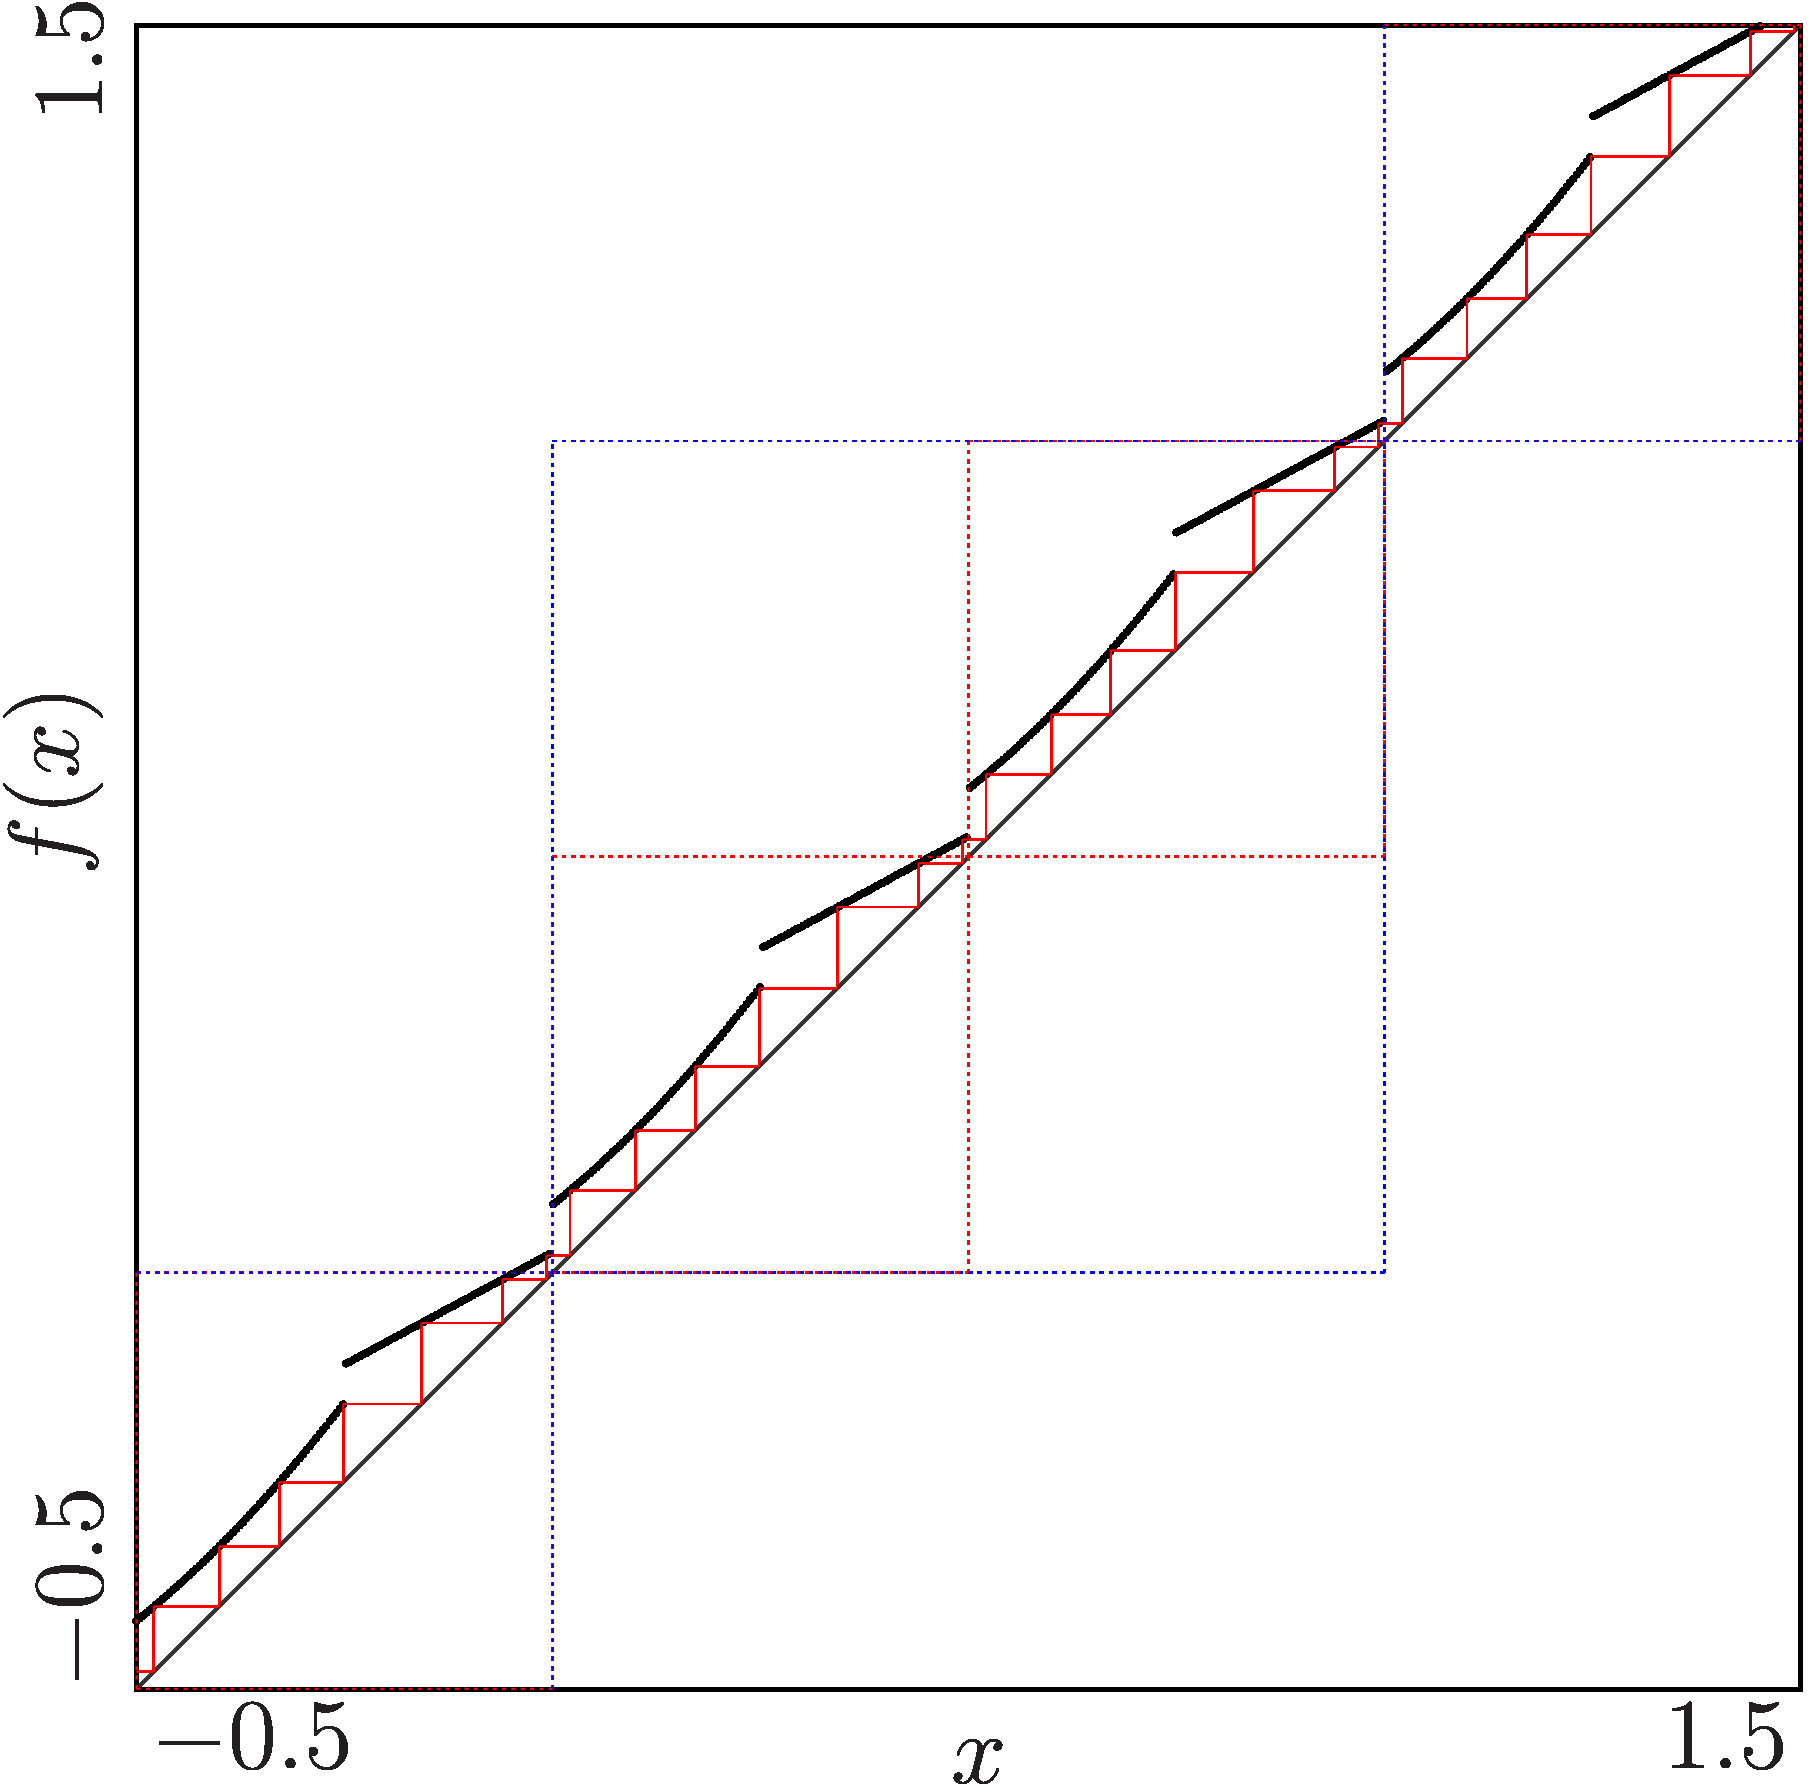
\includegraphics[width=\textwidth]{Figs/archetypal_model_lifted.png}
			\end{figure}
		\end{column}
		\begin{column}{.5 \textwidth}
			\begin{itemize}
				\item Lift the model from $[0, 1)$ to $\mathbb{R}$
				      %\item The lifted model repeats every $1$ step
				      %\item But it even repeats every $\frac{1}{2}$ step because of the built-in symmetry
				\item Drop the model to $[0, \frac{1}{2})$
				\item[$\Rightarrow$] Halved Model
			\end{itemize}
			\begin{align*}
				x    & \mapsto g(x) \mod \frac{1}{2}                                              \\
				g(x) & = \begin{cases}
					         g_L(x) = a_L \cdot x^2 + b_L \cdot x + c_L & \text{ if } x < \frac{1}{4} \\
					         g_R(x) = b_R \cdot x + c_R                 & \text{ else}
				         \end{cases}
			\end{align*}
		\end{column}
	\end{columns}
\end{frame}

\begin{frame}{Period Adding}
	\only<1>{
		\vspace{-1em}
		\begin{figure}
			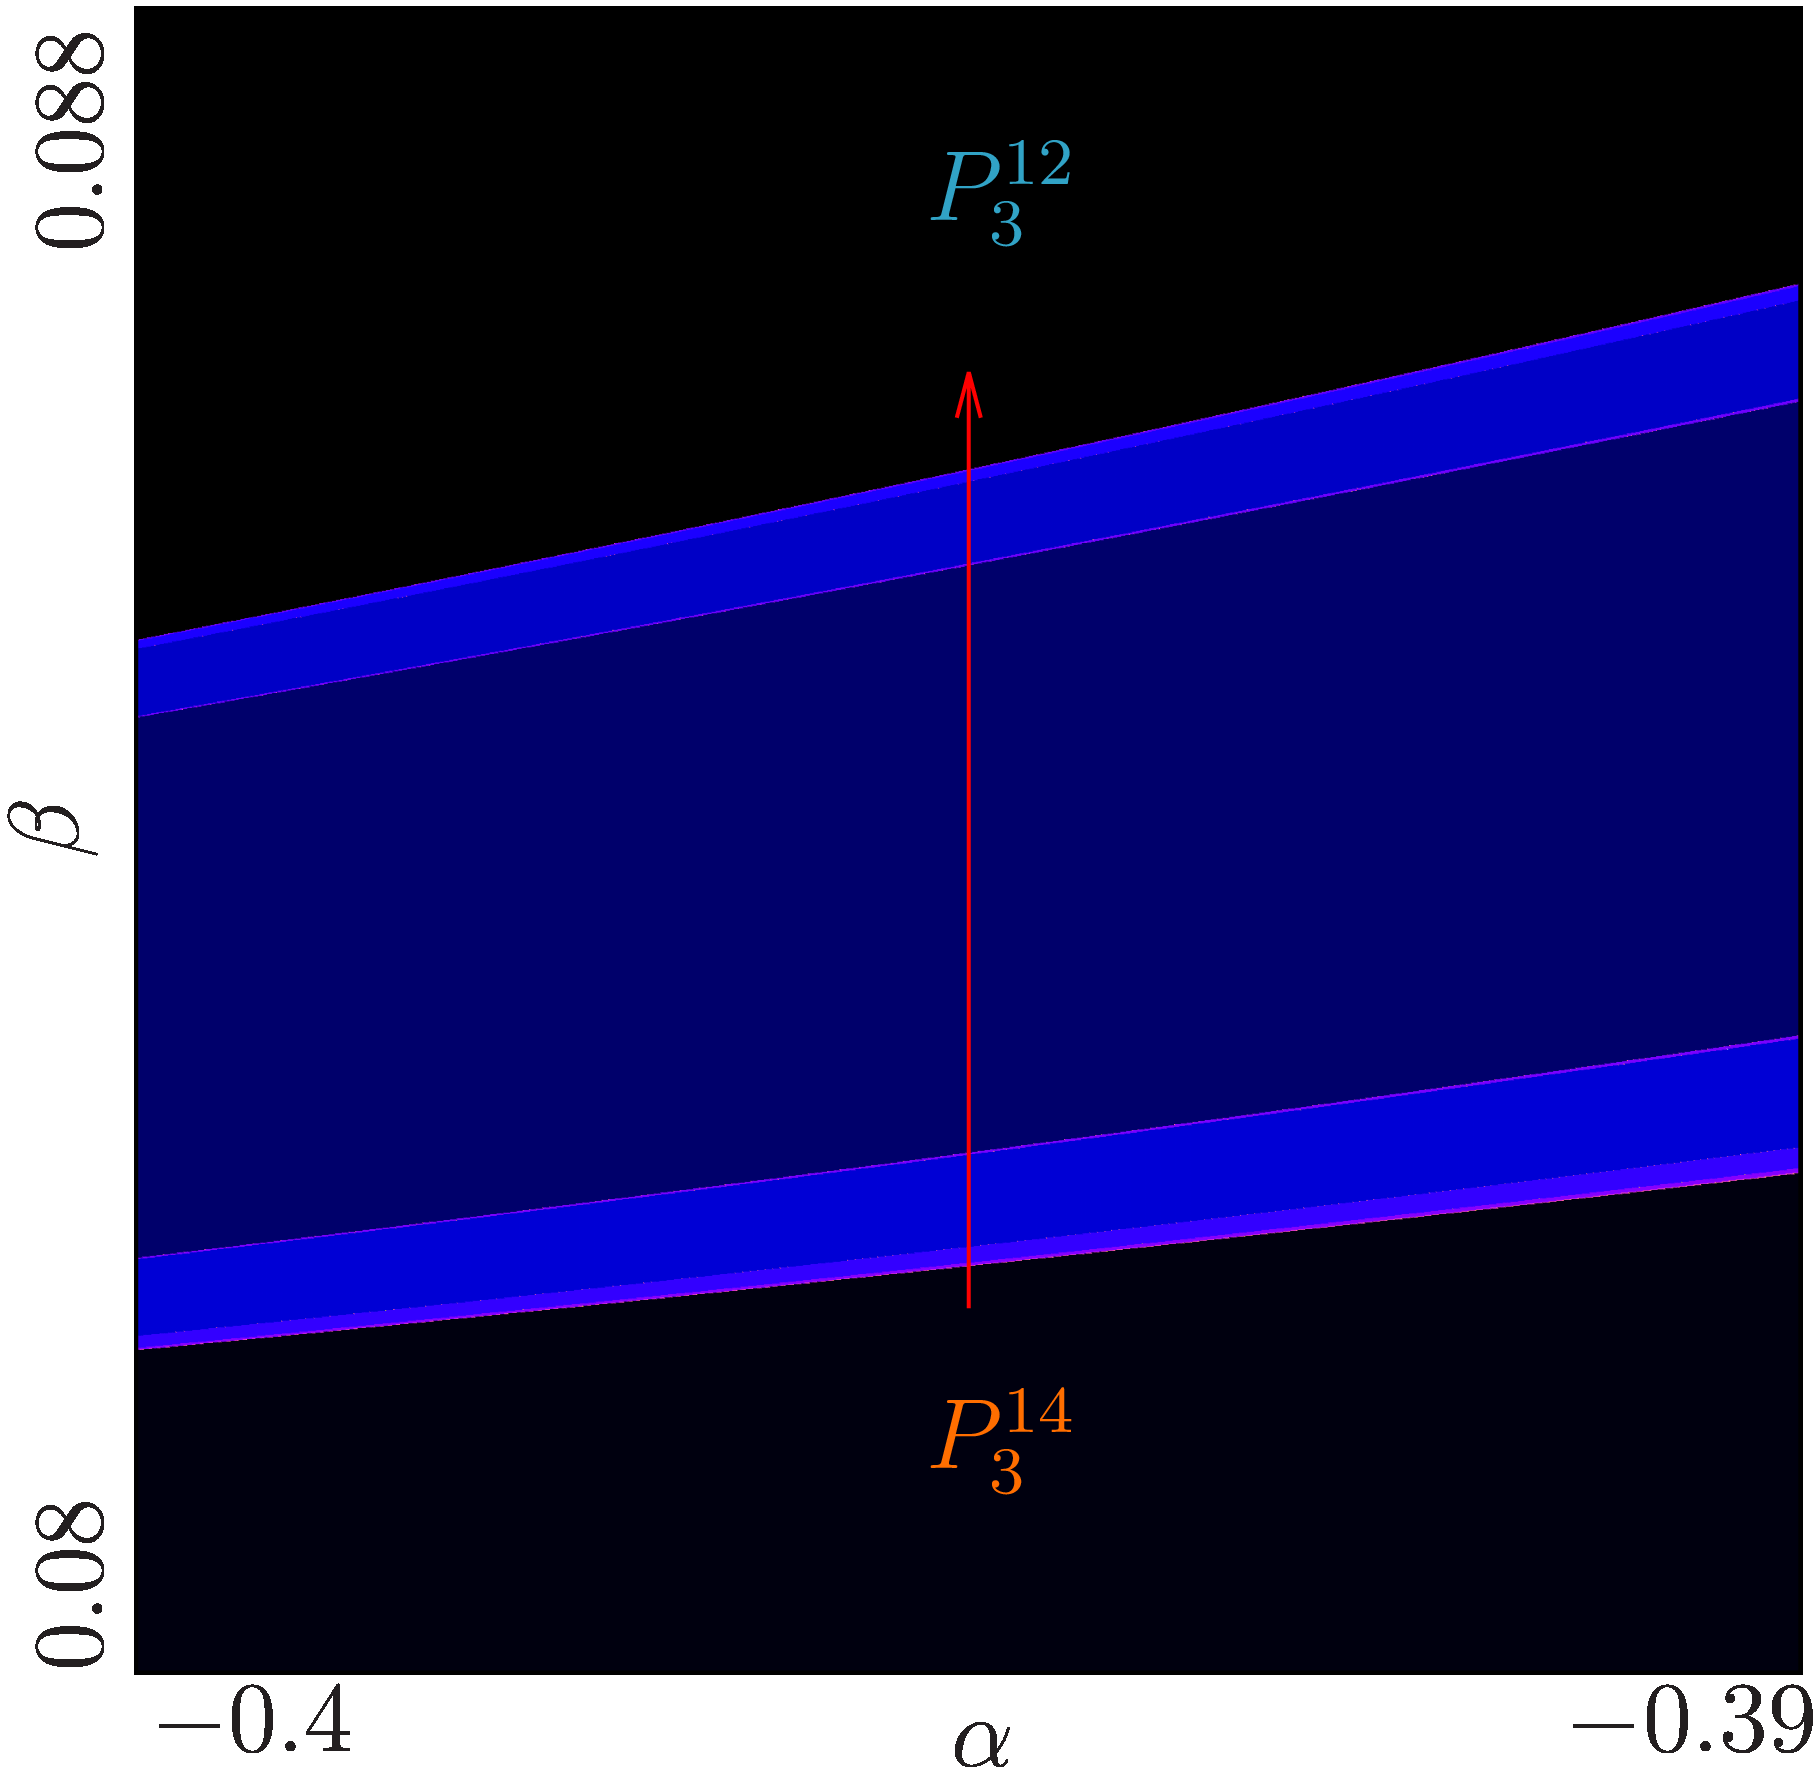
\includegraphics[width=.4 \textwidth]{Figs/archetypal_model_halved_add_hor_2D.png}
			\quad
			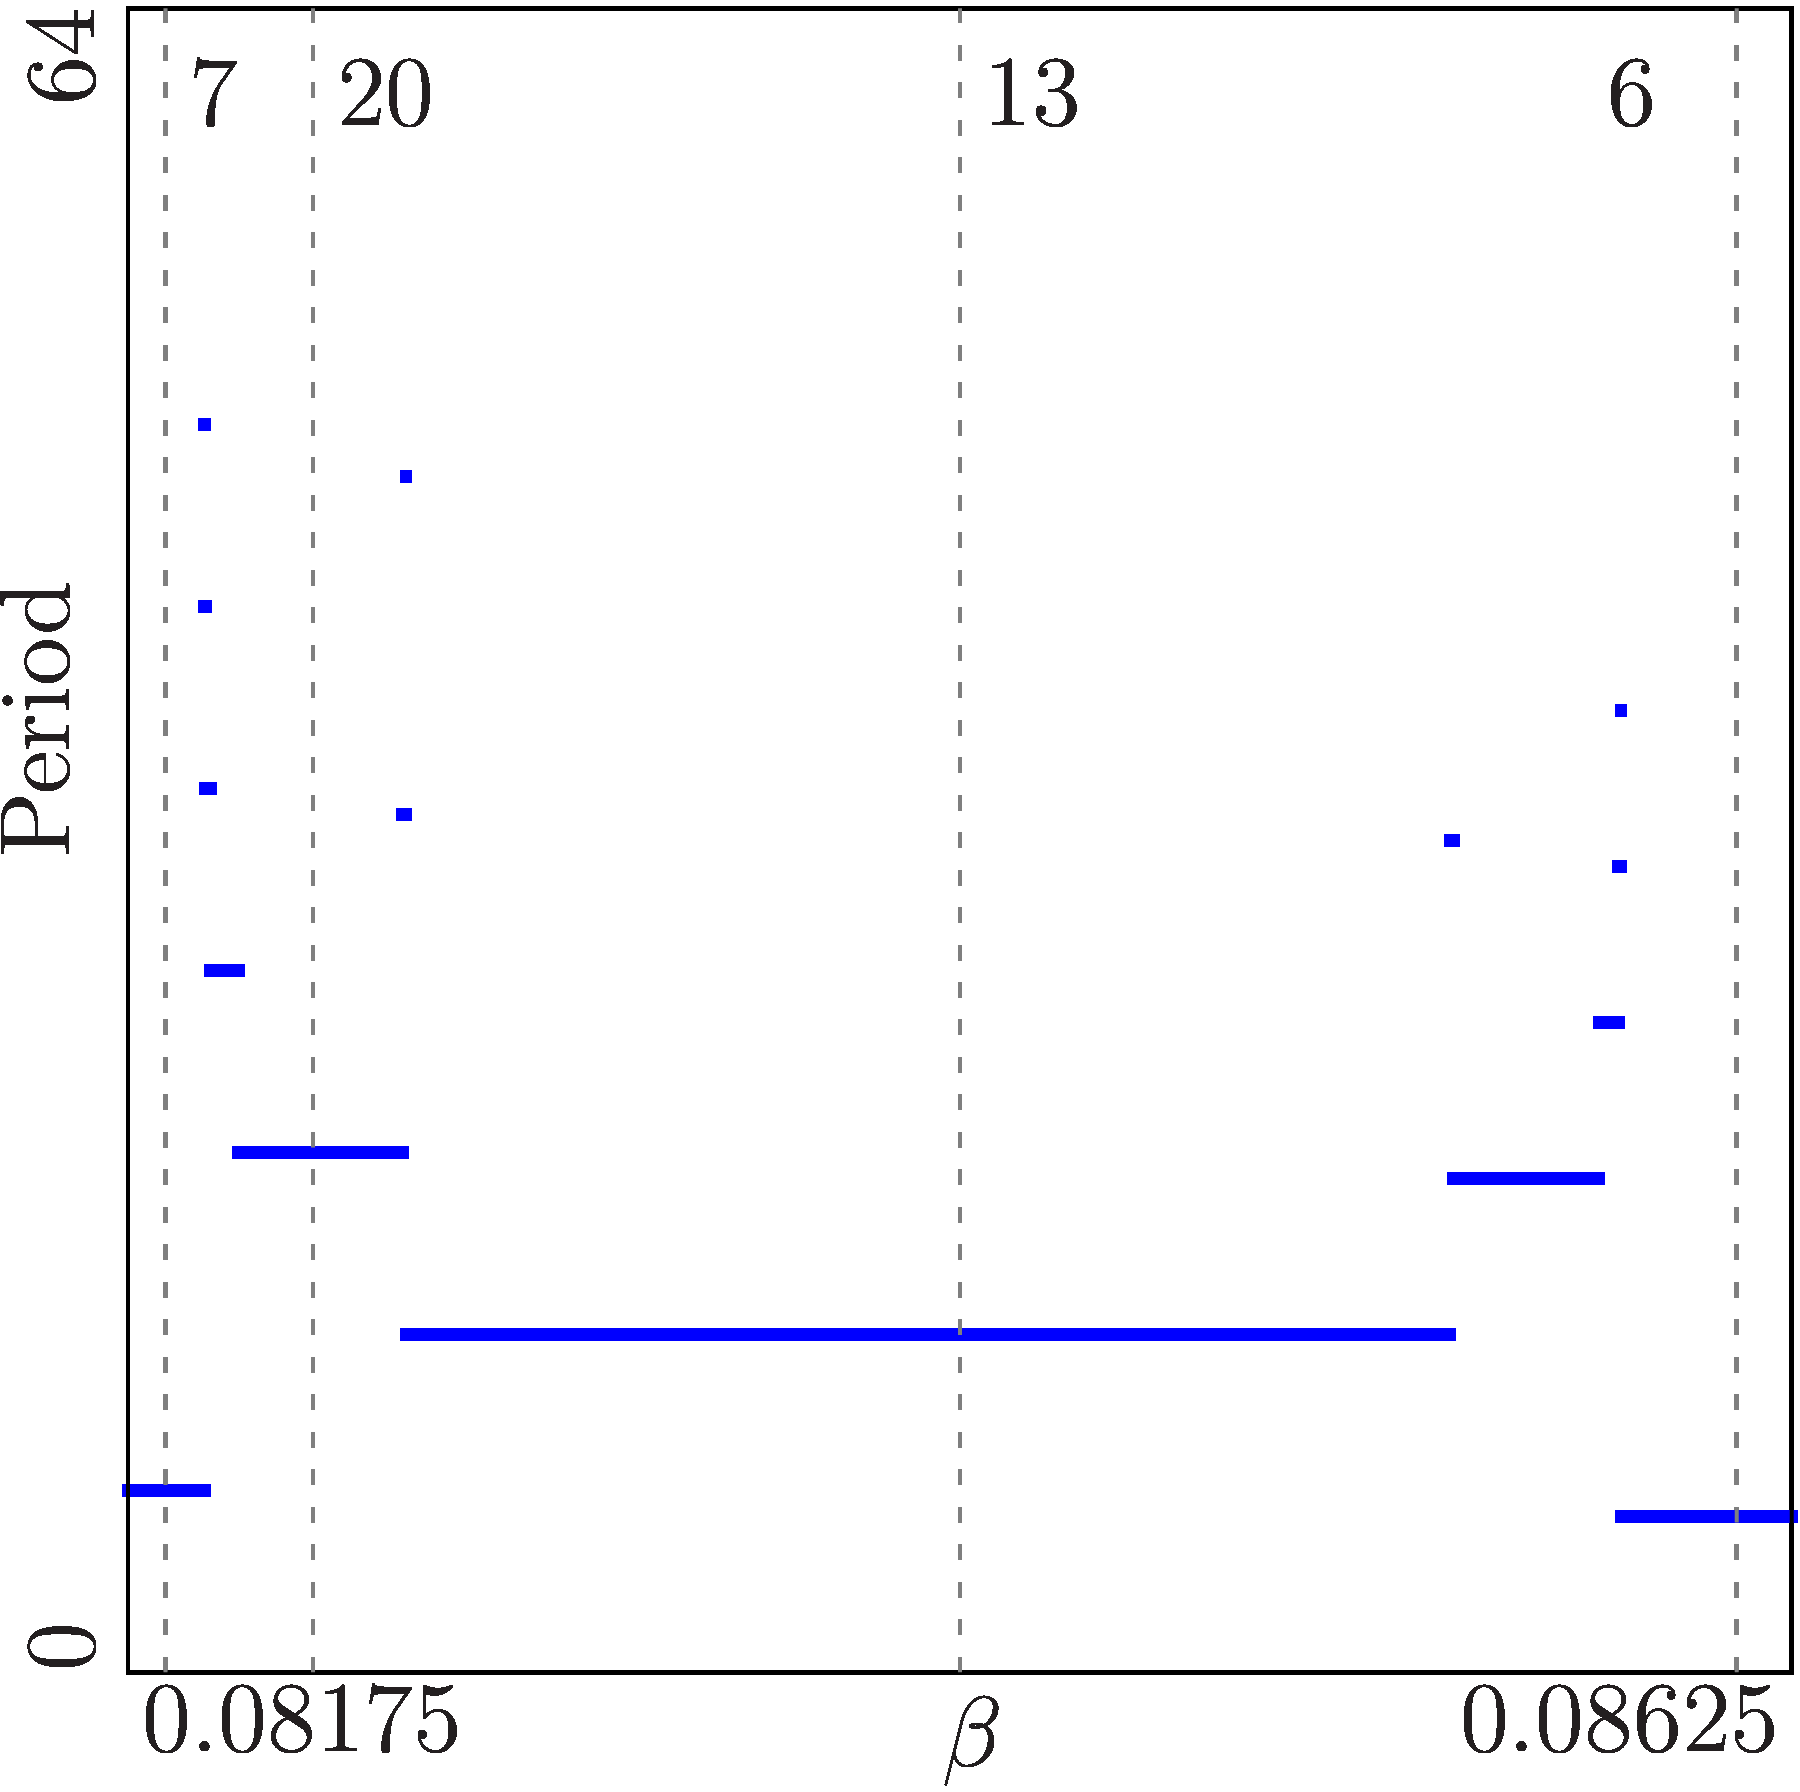
\includegraphics[width=.4 \textwidth]{Figs/archetypal_model_halved_add_hor_1D.png}
		\end{figure}
	}
	\only<2>{
		\vspace{-1em}
		\begin{figure}
			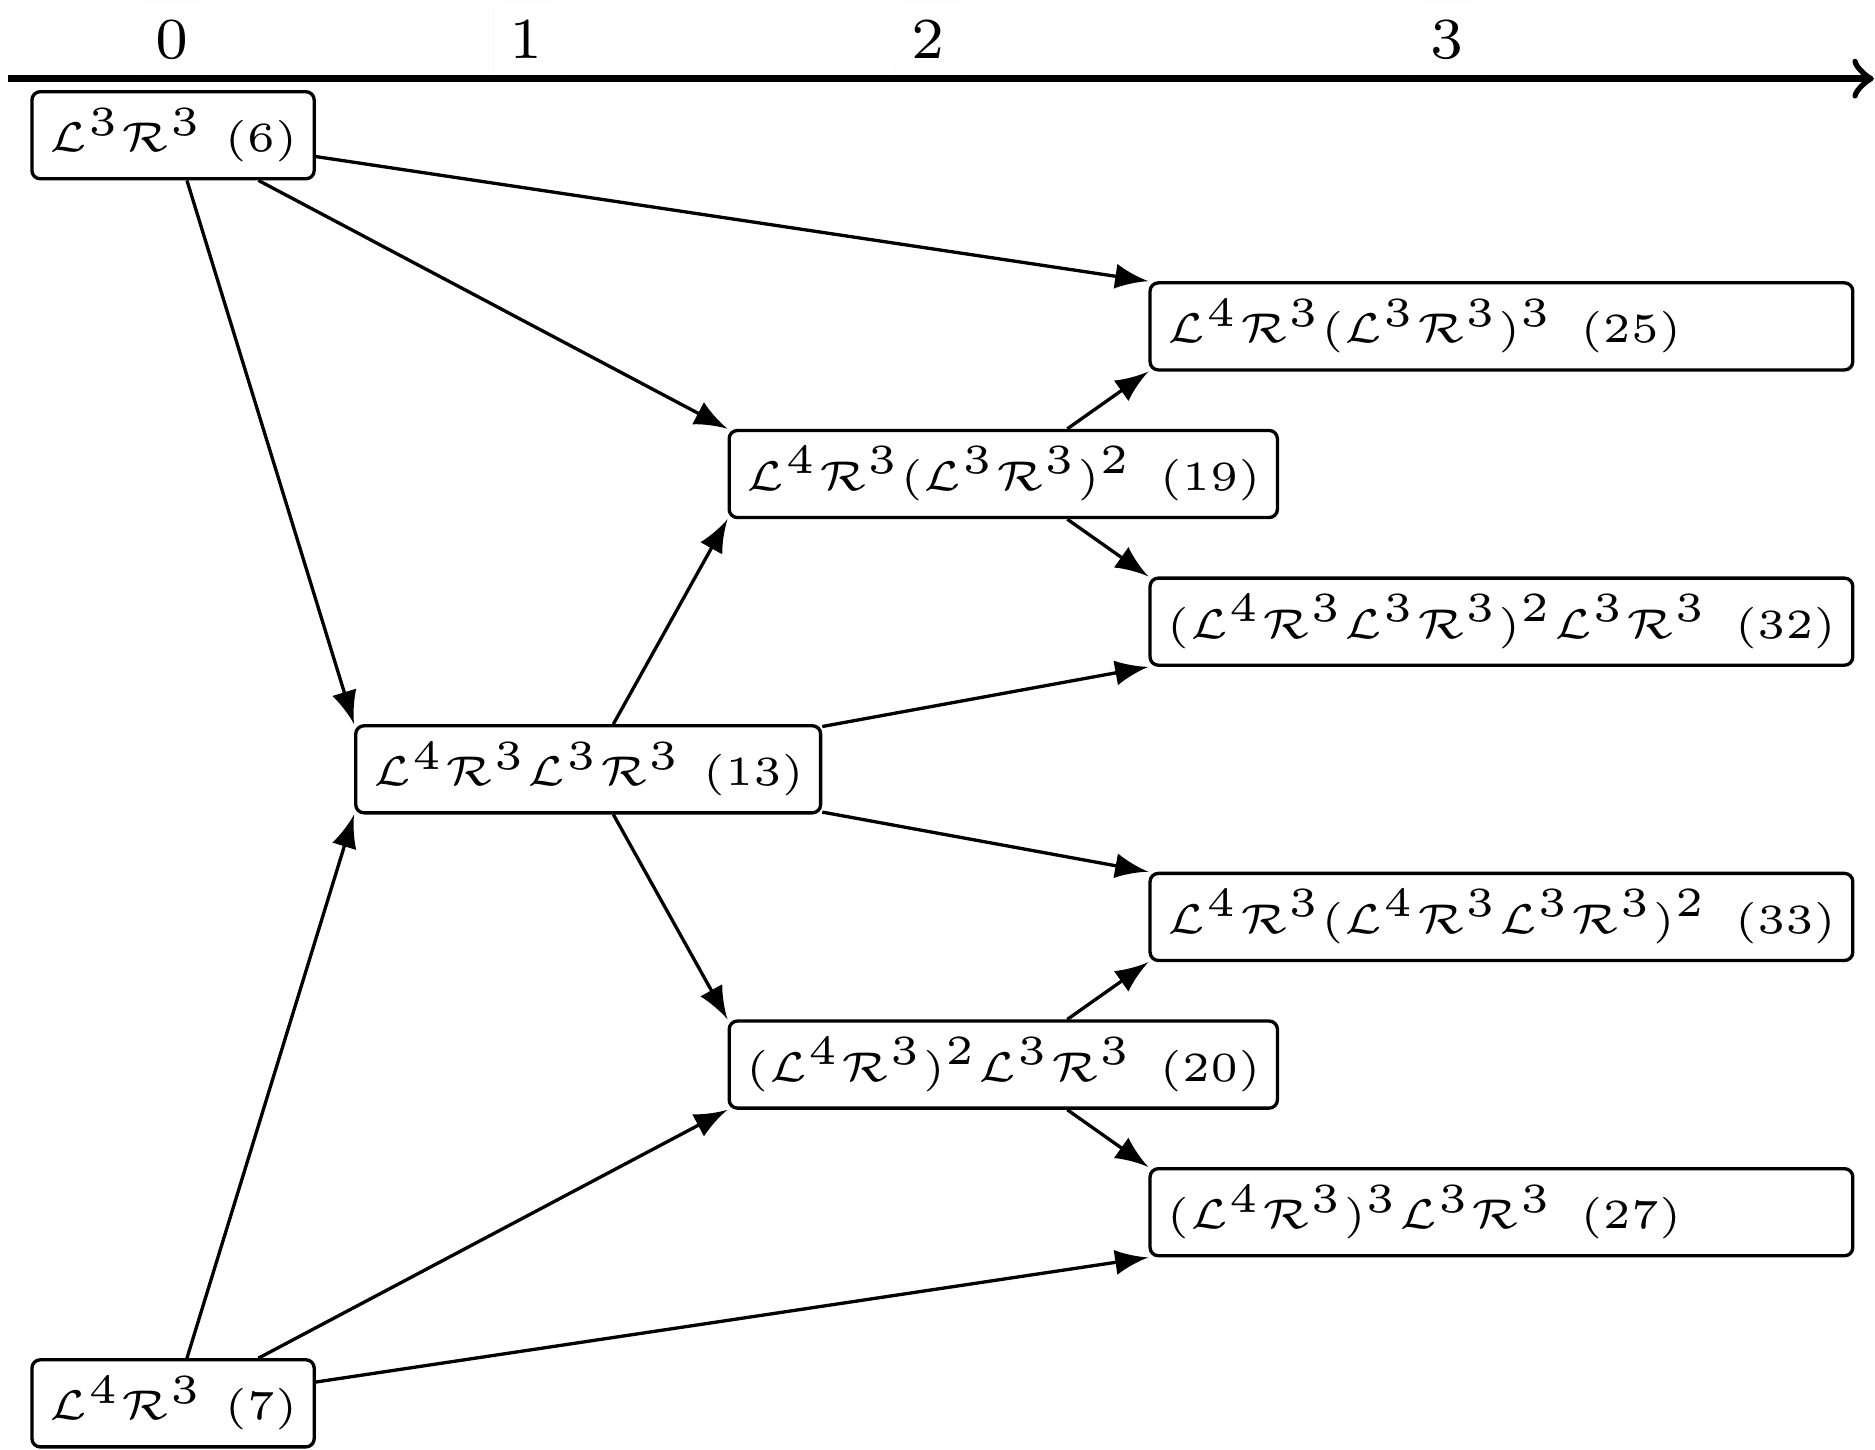
\includegraphics[width=.6 \textwidth]{Figs/Trees/HalvedArchetypal/adding.png}
		\end{figure}
	}
\end{frame}

\begin{frame}{Period Adding Results}
	\vspace{-1em}
	\begin{center}
		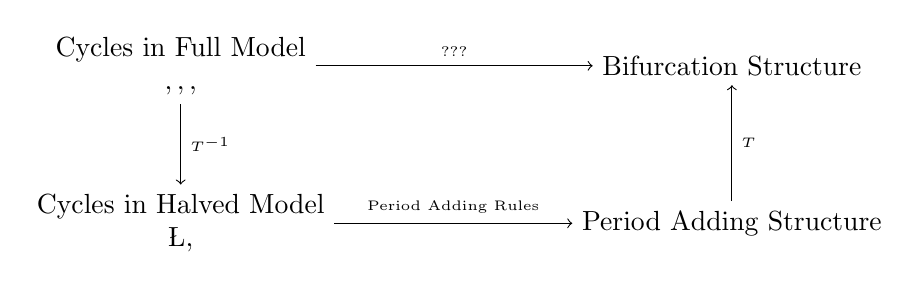
\begin{tikzpicture}[every text node part/.style={align=center}]
			\node (FC) at (0, 2) {Cycles in Full Model \\ $\A, \B, \C, \D$};
			\node (FB) at (7, 2) {Bifurcation Structure};

			\node (HC) at (0, 0) {Cycles in Halved Model \\ $\L, \R$};
			\node (HA) at (7, 0) {Period Adding Structure};

			\draw[->] (FC) -- (HC) node[midway,right] {\tiny $T^{-1}$};
			\draw[->] (HC) -- (HA) node[midway,above] {\tiny Period Adding Rules};
			\draw[->] (HA) -- (FB) node[midway,right] {\tiny $T$};
			\draw[->] (FC) -- (FB) node[midway,above] {\tiny ???};
		\end{tikzpicture}
	\end{center}

	\begin{itemize}
		\item Algorithms for translating cycles between both models
		\item Formal description of novel bifurcation structure
		      \begin{itemize}
			      \item When do cycles coexist?
			      \item Symbolic Sequences
			      \item Periods
			      \item Rotation Numbers (here tuples)
		      \end{itemize}
	\end{itemize}
\end{frame}

\begin{frame}{Translation Type A (Symmetric Cycle)}
	\vspace{3em}
	\centering
	\begin{tikzpicture}[thick,scale=1, every node/.style={font=\huge}]
		\path[draw=none] (0,0) -- (14,-3);
		%
		\coordinate (a) at (7, 0);
		\coordinate (b) at (7, -2.5);
		%
		% A1B2C1D2 -> L1R2
		%
		\only<1-4>{
			\node (cycleA) at (a) {$\A^{1}\B^{2}\C^{1}\D^{2}$};
		}
		\only<2>{
			\draw [decorate,decoration={brace,mirror}] (5.3, -0.8) -- (8.7, -0.8);
			\node at (7, -1.5) {4-Syllable};
		}
		\only<3>{
			\node (cycleB) at (b) {$\L^{1}\R^{2}\L^{1}\R^{2}$};
		}
		\only<4>{
			\node (cycleB) at (b) {$\L^{1}\R^{2}$};
		}
		\only<3-4>{
			\draw[->] (cycleA) -- (cycleB) node[midway,right=0.5em,scale=0.5] {$T^{-1}$};
		}
		%
		% L1R2
		%
		\only<5-8>{
			\node (cycleA) at (a) {$\L^{1}\R^{2}$};
		}
		\only<6>{
			\draw [decorate,decoration={brace,mirror}] (6.0, -0.8) -- (8.0, -0.8);
			\node at (7, -1.5) {2-Syllable};
		}
		\only<7-8>{
			\node (cycleB) at (b) {$\A^{1}\B^{2}$};
		}
		\only<8>{
			\node at (9, -2.5) {???};
		}
		\only<9>{
			\node (cycleA) at (a) {$\L^{1}\R^{2}\L^{1}\R^{2}$};
			\node (cycleB) at (b) {$\A^{1}\B^{2}\C^{3}\D^{4}$};
		}
		\only<7-9>{
			\draw[->] (cycleA) -- (cycleB) node[midway,right=0.5em,scale=0.5] {$T$};
		}
		%
	\end{tikzpicture}

	\vspace{3em}
	\only<4>{
		\begin{itemize}
			\item Remove redundancy if the cycle repeats
		\end{itemize}
	}
	\only<9>{
		\begin{itemize}
			\item If we cannot pair all 2-Syllables $\Rightarrow$ Write the cycle twice
		\end{itemize}
	}
\end{frame}

\begin{frame}{Translation Type B (Asymmetric Cycles)}
	\vspace{3em}
	\centering
	\begin{tikzpicture}[thick,scale=1, every node/.style={font=\huge}]
		\path[draw=none] (0,0) -- (14,-3);
		%
		\coordinate (a) at (7, 0);
		\coordinate (b) at (7, -2.5);
		\coordinate (al) at (3, 0);
		\coordinate (ar) at (11, 0);
		\coordinate (bl) at (3, -2.5);
		\coordinate (br) at (11, -2.5);
		%
		\coordinate (al) at (3, 0);
		\coordinate (ar) at (11, 0);
		\coordinate (bl) at (3, -2.5);
		\coordinate (br) at (11, -2.5);
		%
		% A1B2C3D4 -> L1R2L3R4
		%
		\only<1-2>{
			\node (cycleA) at (a) {$\A^{1}\B^{2}\C^{3}\D^{4}$};
		}
		\only<2>{
			\node (cycleB) at (b) {$\L^{1}\R^{2}\L^{3}\R^{4}$};
			\draw[->] (cycleA) -- (cycleB) node[midway,right=0.5em,scale=0.5] {$T^{-1}$};
		}
		%
		\only<3-7>{
			\node (cycleAL) at (al) {$\A^{1}\B^{2}\C^{3}\D^{4}$};
			\node (cycleBL) at (bl) {$\L^{1}\R^{2}\L^{3}\R^{4}$};
			\node (cycleAR) at (ar) {$\A^{3}\B^{4}\C^{1}\D^{2}$};
		}
		\only<3-6>{
			\draw[->] (cycleAL) -- (cycleBL) node[midway,right=0.5em,scale=0.5] {$T^{-1}$};
		}
		\only<4-7>{
			\node (cycleBR) at (br) {$\L^{3}\R^{4}\L^{1}\R^{2}$};
		}
		\only<4-6>{
			\draw[->] (cycleAR) -- (cycleBR) node[midway,right=0.5em,scale=0.5] {$T^{-1}$};
		}
		\only<5>{
			\draw[->] (cycleBL) -- (cycleBR) node[midway,above=0.2em,scale=0.5] {$s_{2}$};
		}
		\only<6-7>{
			\draw[double equal sign distance] (cycleBL) -- (cycleBR) node[midway,above=0.2em,scale=0.5] {$\equiv_{2}$};
		}
		\only<7>{
			\draw[->] (cycleBR) -- (cycleAR) node[midway,right=0.5em,scale=0.5] {$T$};
			\draw[->] (cycleBL) -- (cycleAL) node[midway,right=0.5em,scale=0.5] {$T$};
		}
		%
	\end{tikzpicture}

	\vspace{3em}
	\only<2>{
		\begin{itemize}
			\item No repetition
		\end{itemize}
	}
	\only<6>{
		\begin{itemize}
			\item Translations of twin cycles are $\equiv_{2}$ equivalent
		\end{itemize}
	}
	\only<7>{
		\begin{itemize}
			\item[$\Rightarrow$] Check all $\equiv_{2}$ equivalent symbolic sequences
		\end{itemize}
	}
\end{frame}

\begin{frame}{Translation: At Most Two Coexisting Cycles}
	\vspace{3em}
	\centering
	\begin{tikzpicture}[thick,scale=1, every node/.style={font=\huge}]
		\path[draw=none] (0,0) -- (14,-3);
		%
		\coordinate (al) at (3, 0);
		\coordinate (ar) at (11, 0);
		\coordinate (bl) at (3, -2.5);
		\coordinate (br) at (11, -2.5);
		%
		\only<1>{
			\node (sigma) at (al) {$\sigma$};
			\node (s4sigma) at (ar) {$s_{4}\left(\sigma\right)$};
		}
		\only<2-5>{
			\node (sigma) at (al) {$\sigma_{1}\sigma_{2} \ldots \sigma_{n}$};
			\node (s4sigma) at (ar) {$\sigma_{3} \ldots \sigma_{n}\sigma_{1}\sigma_{2}$};
		}
		\only<6-9>{
			\node (sigma) at (al) {$\sigma_{1}\sigma_{2} \ldots \sigma_{2k+1}$};
			\node (s4sigma) at (ar) {$\sigma_{3} \ldots \sigma_{2k+1}\sigma_{1}\sigma_{2}$};
		}
		\only<3-5>{
			\node[scale=0.6] (phi) at (bl) {$t\left(\sigma_{1}\sigma_{2}\right) \ldots t\left(\sigma_{n-1}\sigma_{n}\right)$};
			\node[scale=0.6] (s4phi) at (br) {$t\left(\sigma_{3}\sigma_{4}\right) \ldots t\left(\sigma_{n-1}\sigma_{n}\right)t\left(\sigma_{1}\sigma_{2}\right)$};
		}
		\only<1-9>{
			\draw[->] (sigma) -- (s4sigma) node[midway,above=0.2em,scale=0.5] {$s_{4}$};
		}
		\only<4>{
			\draw[->] (phi) -- (s4phi) node[midway,above=0.2em,scale=0.5] {$s_{4}$};
		}
		\only<6>{
			\node[scale=0.5] (phi) at (bl) {$t\left(\sigma_{1}\sigma_{2}\right) \ldots t\left(\sigma_{2k+1}\sigma_{1}\right)  \ldots t\left(\sigma_{2k}\sigma_{2k+1}\right)$};
			\node[scale=0.5] (s4phi) at (br) {$t\left(\sigma_{3}\sigma_{4}\right) \ldots t\left(\sigma_{2k+1}\sigma_{1}\right) \ldots t\left(\sigma_{2k}\sigma_{2k+1}\right)t\left(\sigma_{1}\sigma_{2}\right)$};
		}
		\only<7-9>{
		\node[scale=0.6] (phi) at (bl) {$\phi_{1} \ldots \phi_{k} t\left(\sigma_{2k+1}\sigma_{1}\right) \phi'_{1}  \ldots \phi'_{k}$};
		\node[scale=0.6] (s4phi) at (br) {$\phi_{2} \ldots \phi_{k} t\left(\sigma_{2k+1}\sigma_{1}\right) \phi'_{1} \ldots \phi'_{k}\phi_{1}$};
		}
		\only<5>{
			\draw[double equal sign distance] (phi) -- (s4phi) node[midway,above=0.2em,scale=0.5] {$\equiv_{4}$};
		}
		\only<8>{
			\draw[->] (phi) -- (s4phi) node[midway,above=0.2em,scale=0.5] {$s_{4}$};
		}
		\only<9>{
			\draw[double equal sign distance] (phi) -- (s4phi) node[midway,above=0.2em,scale=0.5] {$\equiv_{4}$};
		}
		\only<3-9>{
			\draw[->] (sigma) -- (phi) node[midway,right=0.5em,scale=0.5] {$T$};
			\draw[->] (s4sigma) -- (s4phi) node[midway,right=0.5em,scale=0.5] {$T$};
		}
		%
	\end{tikzpicture}

	\vspace{3em}
	\only<6-9>{
		\begin{itemize}
			\item Also true for odd $n = 2k + 1$
		\end{itemize}
	}
\end{frame}

\begin{frame}{Translation: No Coexistence when Number of 2-Syllables Odd}
	\vspace{3em}
	\centering
	\begin{tikzpicture}[thick,scale=1, every node/.style={font=\huge}]
		\path[draw=none] (0,0) -- (14,-3);
		%
		\coordinate (al) at (3, 0);
		\coordinate (ar) at (11, 0);
		\coordinate (bl) at (3, -2.5);
		\coordinate (br) at (11, -2.5);
		%
		\only<1>{
			\node (sigma) at (al) {$\sigma$};
			\node (s2sigma) at (ar) {$s_{2}\left(\sigma\right)$};
		}
		\only<2-7>{
			\node (sigma) at (al) {$\sigma_{1}\sigma_{2}\ldots\sigma_{2k+1}$};
			\node (s2sigma) at (ar) {$\sigma_{2}\ldots\sigma_{2k+1}\sigma_{1}$};
		}
		\only<3>{
			\node[scale=0.4] (phia) at (bl) {$t\left(\sigma_{1}\sigma_{2}\right) \ldots t\left(\sigma_{2k+1}\sigma_{1}\right) t\left(\sigma_{2}\sigma_{3}\right) \ldots t\left(\sigma_{2n}\sigma_{2k+1}\right)$};
			\node[scale=0.4] (phib) at (br) {$t\left(\sigma_{2}\sigma_{3}\right) \ldots t\left(\sigma_{2n}\sigma_{2k+1}\right) t\left(\sigma_{1}\sigma_{2}\right) \ldots t\left(\sigma_{2k+1}\sigma_{1}\right)$};
		}
		\only<4-7>{
		\node[scale=0.6] (phia) at (bl) {$\phi_{1} \ldots \phi_{n} t(\sigma_{2k+1}\sigma_{1}) \phi'_{1} \ldots \phi'_{n}$};
		\node[scale=0.6] (phib) at (br) {$\phi'_{1} \ldots \phi'_{n} \phi_{1} \ldots \phi_{n} t(\sigma_{2k+1}\sigma_{1})$};
		}
		\only<5>{
			\draw[->] (phia) -- (phib) node[midway,above=0.2em,scale=0.5] {$s_{4}^{k+1}$};
		}
		\only<6-7>{
			\draw[double equal sign distance] (phia) -- (phib) node[midway,above=0.2em,scale=0.5] {$\equiv_{4}$};
		}
		\only<1-7>{
			\draw[->] (sigma) -- (s2sigma) node[midway,above=0.2em,scale=0.5] {$s_{2}$};
		}
		\only<3-7>{
			\draw[->] (sigma) -- (phia) node[midway,right=0.5em,scale=0.5] {$T$};
			\draw[->] (s2sigma) -- (phib) node[midway,right=0.5em,scale=0.5] {$T$};
		}
		%
	\end{tikzpicture}

	\vspace{3em}
	\only<7>{
		\begin{itemize}
			\item[$\Rightarrow$] No coexistence
			\item[$\Rightarrow$] Periods of translated cycle doubled
		\end{itemize}
	}
\end{frame}

\begin{frame}{Coexistence in Child Nodes}
	\vspace{3em}
	\centering
	\begin{tikzpicture}[thick,scale=1,
			every node/.style={
					draw,rectangle,line width=0.4pt,
					minimum height=2em,minimum width=2em,
					rounded corners=1pt
				}]
		\path[draw=none] (0,0) -- (14,-3);
		%
		\coordinate (c1) at (4, -2.5);
		\coordinate (a1) at (2.5, 0);
		\coordinate (b1) at (5.5, 0);
		\coordinate (c2) at (10, -2.5);
		\coordinate (a2) at (8.5, 0);
		\coordinate (b2) at (11.5, 0);
		%
		\node (a1) at (a1) {\only<2-7>{\tiny odd}};
		\node (b1) at (b1) {\only<2-7>{\tiny odd}};
		\only<3-7>{
			\node[fill=yellow] (c1) at (c1) {\tiny even};
			\draw[->] (a1) -- (c1);
			\draw[->] (b1) -- (c1);
		}
		%
		\only<4-7>{
			\node[fill=yellow] (a2) at (a2) {\only<5-7>{\tiny even}};
			\node (b2) at (b2) {\only<5-7>{\tiny odd}};
		}
		\only<6-7>{
			\node (c2) at (c2) {\tiny odd};
			\draw[->] (a2) -- (c2);
			\draw[->] (b2) -- (c2);
		}
		%
	\end{tikzpicture}

	\vspace{3em}
	\only<7>{
		\begin{itemize}
			\item Both parents with coexistence will never happen (for this structure)
		\end{itemize}
	}
\end{frame}

%%% Local Variables:
%%% mode: latex
%%% TeX-master: "../Vortrag_Frauenhofer_Weik"
%%% End:
